\documentclass[10pt,aps,onecolumn,floatfix,notitlepage,nofootinbib,showkeys]{revtex4-2}
\usepackage{amsmath,amssymb,mathtools,bm}
\usepackage{booktabs}
\usepackage{graphicx}
\usepackage{hyperref}
\hypersetup{hidelinks}
\usepackage{array}
\usepackage{microtype}
\usepackage{xcolor}
\usepackage{tikz}
\usetikzlibrary{arrows.meta,calc,positioning}
\newcommand{\vk}{\bm{k}}
\newcommand{\ve}{\bm{e}}
\newcommand{\vf}{\bm{f}}
\newcommand{\vu}{\bm{u}}
\newcommand{\vF}{\bm{F}}
\newcommand{\vR}{\bm{R}}
\newcommand{\vx}{\bm{x}}
\newcommand{\vp}{\bm{p}}
\newcommand{\vd}{\bm{d}}
\newcommand{\vg}{\bm{v}_{g}}
\newcommand{\vJ}{\bm{J}}
\newcommand{\vq}{\bm{q}}
\newcommand{\vpsi}{\bm{\psi}}
\newcommand{\vchi}{\bm{\chi}}
\newcommand{\veta}{\bm{\eta}}
\newcommand{\vrr}{\bm{r}}
\newcommand{\vt}{\bm{t}}
\newcommand{\ex}{\hat{\bm{x}}}
\newcommand{\ey}{\hat{\bm{y}}}
\newcommand{\ez}{\hat{\bm{z}}}
\newcommand{\order}{\mathcal O}
\newcommand{\Ic}{\mathcal I_c}
\newcommand{\Cc}{\mathcal C}
\newcommand{\Lambdab}{\Lambda_b}
\newcommand{\BZ}{\mathrm{BZ}}
\newcommand{\qT}{\mathrm{qT}}
\newcommand{\qL}{\mathrm{qL}}
\newcommand{\PqT}{P_{\mathrm{qT}}}
\newcommand{\PqL}{P_{\mathrm{qL}}}
\newcommand{\PAone}{P_{A_1}^{(c)}}
\newcommand{\Tr}{\operatorname{Tr}}
\newcommand{\ImH}{\operatorname{Im}_{\!H}}
% Number sections and subsections consistently in headings and cross-references.
\renewcommand{\thesection}{\arabic{section}}
\renewcommand{\thesubsection}{\thesection.\arabic{subsection}}
\makeatletter
\def\p@subsection{}
\makeatother
\ifdefined\pdftrailerid\pdftrailerid{}\fi
% Source identity and validation scope (comments only; no typeset content).
% Working edition: end matter following the approved Section IX, 11 November 2026.
% PACKAGE_SHA256SUMS.json records the files in this cumulative package.
% checks/BUILD_CHECK.json identifies the corresponding main and supplemental build.
% checks/IX_APPROVED_CLAIMS.json and checks/VIII_CERTIFICATES.json distinguish the
% original reference-taper certificate from the separate bounds for the increasing ramp.
% These scientific inputs and bounds are retained in the present editorial revision.
% The following comments are historical. Each edition label and hash refers to its own release.
% Current edition: checked corrections and prediction-evidence revision, 28 September 2026 (Toronto).
% Current source identities, applied edits and completed checks: checked_revision_manifest.json.
% Exact manuscript changes: checked_revision_edits.json (40 spans:17 main,23 supplement;39 reported plusC17 angular path).
% Main and supplement retain onecolumn. Historical numerical table entries are preserved.
% The branch-edge proof, local definitions, navigation and evidence wording follow the checked report.
% New and preceding check records are identified in EVIDENCE_ACCESS.md and evidence/.
% This source update does not enlarge the fixed-frequency R8 certificate.
% Original GB producer history and factual author/disclosure/public-release items remain bounded open matters.
% All previous source-binding text is preserved below as historical provenance.
% ---- Preserved preceding source-binding records follow ----
% Current edition: two-perspective framing revision, 27 September 2026 (Toronto).
% Current source identities and checks: two_perspective_framing_manifest.json.
% Exact changes: two_perspective_framing_edits.json (E1-E3, three main prose spans).
% Abstract and supplement unchanged; both documents retain onecolumn.
% No numerical recertification, new clock model, or enlargement of claim scope.
% All earlier source-binding text is preserved below as historical provenance.
% ---- Preserved preceding source-binding records follow ----
% Current edition: final referee revision, 27 September 2026 (America/Toronto).
% Current identities/checks: referee_revision_manifest.json.
% Exact manuscript replacements: referee_revision_edits.json (14 spans).
% Main and supplement remain single-column. No broad cuts or relocations.
% Selected display rounding and shell-estimate wording do not rerun or enlarge R8.
% Factual author/release/disclosure tasks remain open as stated in the report.
% All earlier records below describe their historical editions.
% ---- Preserved previous source-binding records follow ----
% Current revision: 27 September 2026, four contribution-clarity edits E1--E4.
% Current file identities and completed checks: contribution_clarity_revision_manifest.json.
% Exact manuscript replacements: contribution_clarity_edits.json (4 spans).
% Only main-paper prose changes; the supplement and scientific results are retained.
% This revision does not rerun or extend the R8 certificate.
% Earlier records below describe their own historical editions.
% ---- Preserved previous source-binding record follows ----
% Current revision: 27 September 2026, minimum current-issues corrections.
% Current file identities and completed checks: current_issue_revision_manifest.json.
% Exact manuscript replacements: current_issue_edits.json (10 spans).
% Earlier records below are historical, not identities of this revision.
% Both documents remain single-column; no scientific equations/results changed.
% This revision does not rerun or extend the R8 certificate.
% ---- Preserved earlier source-binding record follows ----
% Editorial shortening and clarity revision implemented, 27 September 2026.
% Current source hashes and all applied edit IDs are recorded in
% editorial_revision_manifest.json; editorial_edits.json supplies exact spans.
% This is a source/layout revision, not a new numerical validation or an
% extension of the R8 certificate. Scientific equations/results retain their
% stated evidence and scope. The comments below and the unchanged
% prediction_integration_manifest.json are historical baseline records.
% ---- Preserved prediction-integration and earlier provenance below ----
% Prediction-integrated manuscript build, 27 September 2026.
% The record below is retained baseline provenance, not a hash description
% or certification of the prediction-integrated sources. See the accompanying
% integration manifest for their current hashes and change record.
% R8 has not been rerun or expanded to certify these new predictions.
% ---- Preserved baseline provenance begins below ----
% Paper One source correspondence: focused revision, 26 September 2026.
% This file is intentionally comments only. It changes no typeset content.
% Compile from this directory: latexmk -pdf paper1_main.tex
% and: latexmk -pdf paper1_supplement.tex
% Alternatively, run pdflatex on each source until references stabilize.
% Both bibliographies are explicit; latexmkrc disables unnecessary BibTeX.
%
% Baseline: PAPER1_LATEX_BUILD_2026-09-26(2).zip.
% Supporting validation: PAPER1_VALIDATION_INTEGRATED_R8(1).zip.
% R8 and its validator are unchanged. Its exact-source check validates its
% archived manuscript/candidate, not these revised TeX files.
% This record associates unchanged mathematics/results with that evidence;
% hashes establish file identity, not a new numerical certification.
% All 185 original displayed math blocks and all eight original tables are
% retained byte-for-byte and in order. No original section or label is lost.
% Original figure data are retained. The selector receives styling changes;
% the additional spectrum displays the existing 49 ACTIVE85 frequency rows.
% The three new displayed formulas and continuum interference table explain
% or evaluate existing source and spectral constructions. Their scope is
% stated in main Secs. IV-VI and supplement SM4; they do not enlarge the
% certified frequency/coupling domain or assert a new continuum-limit proof.
% Main and supplement retain their conditional observer/clock explanations.
% Public archive citation and genuine author contact details remain pending
% as stated in the manuscript. No public deposit is implied by this record.
%
% SHA-256 of original attached sources:
% paper1_main.tex bb1a14bed6775ee6011643aa830cc7cc0c84a7418bc6a1b9c1314276eb8d2dc9
% paper1_supplement.tex bf687d7424050fefd9571072c1fbf4fb24db90690cdcdfd6b0ab85696fcc3786
% SHA-256 of R8 candidate sources:
% manuscript/candidate/paper1_main.tex b6e94ea9f60b27bb428085f1fb6a027bbfbdb0831d3fdcd13dae128fc97dc58f
% manuscript/candidate/paper1_supplement.tex d9b77cfbc9053b2087d1d06dd8032add3e72465ab890602da182d977a4c255a9
% Existing R8 input authority for the added spectrum:
% legacy_rc4/validation/current_numerics/analysis/resolution_execution/robustness/ACTIVE85.json
% sha256 93ae058159343720a54fb272b2d9f9dd5b0cce839d652bf1e0e66f69b8174ef5
% Additional diagnostic records from the reassessment (outside unchanged R8):
% continuum_weak_results.json 21ab02f827e73c22cd6ee8762f1535407202aa8881803730026a1e5496d56d3d
% weak_crosscheck_results.json 449e088b87df319244c27c852f7feaf519d39d52825d306a1a6feb6e5773e90e
% These new diagnostics are specified by the formulas, normalizations,
% source parameters, and quadrature ladders given in supplement SM4.
% They are not claimed to be pre-existing outputs of the R8 validator.
% SHA-256 of final build inputs, excluding this self-describing file:
% aps10pt4-2.rtx 0cc5d7fab6ffd59ba5779f9ddfad990cb8a71438ea390277bafff1824bbcb8e4
% aps4-2.rtx 52d33501cae6dfdf339efeb2a79fda0a2780d1d39d96b61a1c6a6311da6ca05e
% figures/Halpha_transmission_scan_p06.png 04948c9231a539082d234c3af2a68e7d10d560e42f9c6f2e51f589053235cb3d
% figures/continuum_lattice_share_comparison_p06.png e2323d751a32fdfb30f7c39acb5ab33d349e41b0f773cca8d3bd7f14d30e7e02
% figures/paper1_frequency_partition.pdf a446ec83b61e2b8c6c70c6f638c9e95d60ffa74b3b8967304ce45ce392636aa5
% figures/paper1_sectionIV_fig3_bulk_modes_symmetry_v2.pdf 9882955f2a34701f5154841c2325fff32d3344f619e7a1438d2a8672c56575b8
% figures/paper1_sectionVII_fig6a_qT_window_v2.pdf b5de298d32a530958519505a607765331a569cb3de6ef18c6a1e133c5be3836d
% figures/paper1_sectionVII_fig6b_selector_controls_v2.pdf 0d5cfcb0ad6f88ea1c6b4fc6c4cedc282acf52728af4ffc8f7ffe4216642411a
% figures/paper1_sectionVI_fig4_reference_partition_v2.pdf 7c5313c544de0373b3e234355c143d404ec3c569efcd946d7e477b47798f67c1
% latexmkrc abed4d537fbfeeac0ef306877b6a97528125588e4a2344f07e79cab771bc2b0c
% paper1_main.tex de18909953cd48e9828af791d7c755cdf63eefc84d3b6ce9c4d22151de3d36b0
% paper1_methods_references.tex e219c707377f6ed3c2c86cffd6a7cffc9f358cbcb9a334450dad7127de9b8d08
% paper1_supplement.tex e4cf3a1573c3583bab964eccb0e5b93b266aa635cd08926e766b10c9e47f6186
% revsymb4-2.sty 7614d7446d929f49917e54c8590d7ff7408572a9d2d293d209ea718540947d3e
% revtex4-2.cls 58727044fa47fff2663615774f8f24baab978944bbc55f84f8dc08ef91f67358

\begin{document}
\title{Low-Frequency Radiation at a Reciprocal Junction between a Line and a Three-Dimensional Harmonic Lattice}
\author{Mike Fernandes}
\email[Corresponding author: ]{mike1fernand@gmail.com}
\affiliation{Independent Researcher, Ontario, Canada}

\begin{abstract}
Which features of three-dimensional shear radiation from a one-dimensional compression wave depend on the contact? A mechanical picture of discrete space motivates this effective spring model. A line continues between identical leads through a finite passive contact embedded in an infinite harmonic lattice. Eight equally stiff inclined springs couple each active segment to four bulk sites. One Hamiltonian determines the contact forces and their reaction on the line. Only the line wave is incident. Radial source forces sum to zero over each segment's four bulk sites. At long wavelengths, static balance fixes the leading net axial force, whose transverse projection excites shear for oblique wavevectors. With equal positive axial and face-diagonal bulk stiffnesses, both lower modes approach shear polarization. As frequency vanishes at fixed coupling, reflection approaches unity. The incident-power fractions entering this quasi-transverse pair and longitudinal-like upper branch vanish as frequency squared, yet the pair carries $91.2\%$ of bulk emission. Line impedance, bulk density and sound speeds fix both coefficients for each nonzero, nonnegative stiffness profile. Convergence is uniform at fixed positions and fixed positive total stiffness. Static force moments set the profile-dependent part of the emitted share's quadratic correction. At dimensionless frequency $1.2$, a six-segment ramp driven from its softer end converts an estimated $73.6\%$ of incident power into the pair, with conversion guaranteed above $69\%$ throughout independent $\pm5\%$ variations of six segment stiffnesses. In packet simulations starting with the bulk at rest, mean stored shear-like energy divided by initial line energy agrees with spectrum-weighted scattering predictions.
\end{abstract}
\keywords{Lattice dynamics, elastic wave radiation, mode conversion, scattering, lattice Green functions, low-frequency asymptotics}
\maketitle

\section{Introduction}
\label{sec:scope}

When a longitudinal line wave radiates into a three-dimensional lattice, what does force balance fix and what depends on the contact? Motivated by a mechanical picture of discrete space, we prescribe a line with one axial displacement per site, an incident longitudinal wave, the harmonic bulk and the joining springs. We calculate which bulk modes are excited and how much power they carry. On each active line segment, eight inclined central-force springs of equal stiffness form a complete motif. One spring joins each endpoint to each of four surrounding bulk sites. With those sites at equilibrium, extending the segment about a fixed midpoint pulls them inward. Compression reverses the radial forces, whose vector sum is zero.

At long wavelengths, static force balance fixes the leading net force transmitted to the bulk by the loaded contact. This axial force has a component perpendicular to an oblique wavevector and can therefore excite shear motion. With equal axial and diagonal bulk stiffnesses, the lower two acoustic branches approach the two shear polarizations in this limit. We call the pair quasi-transverse (qT) where it is separated from the upper, quasi-longitudinal (qL) branch. At finite wavelength qT polarizations can depart from exact transversality.

Consider an unbroken line with identical leads and a fixed finite set of possible contact positions. For fixed coupling, lattice spacing and equal positive axial and diagonal bulk stiffnesses, the qT and qL fractions of incident line power, summed over emission directions, vanish as $\omega^2$ (Sec.~\ref{pred:sec-lowfreq}, Eq.~\eqref{pred:eq-lowfreq}). Line impedance, bulk mass density and the corresponding sound speed fix each coefficient for every nonnegative stiffness profile with at least one active complete motif. At fixed positive total strength, the fractions divided by $\omega^2$ converge uniformly over profiles on those positions. Reflection tends to unity. Static force moments set the profile-dependent part of the quadratic correction to the fraction of total emitted bulk power carried by qT modes. This fraction tends to about $91.2\%$ and approaches that limit from below for one active motif. A weak-coupling crossover explains why the order of the zero-frequency and zero-coupling limits matters for reflection.

Related questions arise in elastic support loss and wire--bulk phonon transmission. Chang and Geller derive quadratic transmission from the normal end traction of a longitudinal wire mode, and Wilson-Rae resolves the shear contribution from beam compression~\cite{ChangGeller2005,WilsonRae2008}. Atomistic Green functions describe a nanowire between bulk contacts~\cite{ZhangMingoFisher2007}, and scattering matrices describe silicon wire--bulk thermal transport~\cite{DucheminDonadio2011}. For a vector chain coupled to a surface atom of a semi-infinite three-dimensional fcc lattice, Panzer and Goodson calculate total transmission by incident polarization~\cite{PanzerGoodson2008,PanzerGoodson2011Erratum}. Shi \textit{et al.}\ resolve longitudinal nanotube input into longitudinal and out-of-plane flexural waves in graphene~\cite{Shi2018}. Here the line continues through a distributed contact in an infinite lattice, and both leading bulk radiation coefficients are independent of how stiffness is distributed among the complete motifs.

Longitudinal and shear bulk waves separate in an isotropic homogeneous continuum. In a two-dimensional discrete Lamb problem, a longitudinal wave interacting with the free surface generates a head shear wave~\cite{Aleksandrova2014}. Interfaces, terminations, resonators and line defects can mix elastic branches~\cite{ZulKarnain2020,Chaplain2020,NievesSharma2024,Clark2025,DalPoggetto2025}. Graded media convert longitudinal to shear waves, and normal-force exciters direct shear radiation, including in three dimensions~\cite{Boddapati2026Graded,Liang2026MetaExcitation,Lu2026ThreeDimensional}. Chiral lattices couple longitudinal motion, shear and rotation through inclined links~\cite{Mangach2024}. A discrete-chain preprint relates local force matrices to polarization scattering~\cite{GonzalezRamirez2026}. Continuum precedents include axial-force and radial-pressure line sources~\cite{Aldridge1998}, reciprocal tube-wave radiation~\cite{Burridge1993}, and oscillators coupled through an elastic half-space~\cite{Pu2021}.

Incident qT conversion and emitted qT share divide the same qT power by incident line power and total emitted bulk power, respectively. At equal total stiffness, conversion can rise while the share falls (Table~\ref{tab:s6-equal-total}). Collected conversion retains the incident denominator and selects qT power by energy-flow direction, which can differ from the wave normal~\cite{Spies1994,Bacigalupo2018} (Sec.~\ref{pred:sec-collection}).

Finite-frequency conversion depends on the stiffness profile. At $\omega=1.2$ in the units of Sec.~\ref{sec:s2-units-nullspaces}, an increasing ramp selected from a finite scan converts an estimated $73.6\%$ of incident line power into qT modes when driven from its softer end. Its total spring stiffness and peak link stiffness exceed those of a symmetric six-segment reference taper. At the ramp's total stiffness, the reference taper with tripled link stiffnesses and a uniform contact give estimated conversions of $62.7\%$ and $67.8\%$, respectively. Peak link stiffness differs across these three profiles (Table~\ref{tab:s6-coupling-comparison}). At this frequency ramp conversion stays above $69\%$ when the six motif strengths vary independently by up to $5\%$ (Sec.~\ref{sec:s9-robustness}).

Vanel \textit{et al.}\ derived Green-function asymptotics near critical frequencies for scalar square and cubic lattices and applied the approach to a three-dimensional elastic frame~\cite{Vanel2016}. Here we use mode-resolved Green-function and scattering methods~\cite{Ong2018,Sadasivam2017,Khodavirdi2024} to retain the response of the infinite vector lattice at the contact. Section~\ref{sec:s6-controls} tests the axial and radial couplings using separate controls.

Here \emph{generation} means positive outgoing qT power with only the line wave incident and no imposed transverse drive. One autonomous Hamiltonian gives the contact forces on the bulk and their reaction on the line. An independent packet test evolves a finite open truncation of this model with zero initial bulk displacement and velocity. It compares mean stored qT energy divided by initial line energy with the spectrum-weighted scattering prediction (Sec.~\ref{sec:s7-direct}).

We describe motion in equilibrium lattice coordinates and use the Hamiltonian time $\tau$ to report frequencies and powers (Sec.~\ref{sec:s2-geometry}). Supplementary Material Sec.~SM6 gives the conditions for reporting this motion in an internal clock's time.

\section{Effective discrete harmonic model}
\label{sec:s2-model}

An infinite line with one axial displacement per site carries the incident longitudinal wave. Over a finite contact, paired central-force springs couple it to one infinite three-dimensional lattice with a vector displacement at each site. We specify the equilibrium geometry, masses and spring stiffnesses, including the stiffness profile along the contact. The homogeneous bulk dynamical matrix determines the bulk modes. We prescribe the incident line wave as an asymptotic condition. A single autonomous Hamiltonian then determines the contact forces, their reaction on the line and the power radiated into the bulk modes. We use the harmonic expansion about equilibrium and the Bloch description of the periodic bulk~\cite{BornHuang1954,Maradudin1971}.

\subsection{Reference geometry and degrees of freedom}
\label{sec:s2-geometry}

At equilibrium, four existing bulk sites form a square in the plane midway between the endpoints of each active line segment. One inclined spring runs from each endpoint to each corner. The resulting eight springs constitute one complete motif and share a per-spring stiffness $g_i$ on segment $i$. Figure~\ref{fig:sectionII_geometry} shows the geometry. We use $\tau$ for the Hamiltonian evolution parameter.

For stationary scattering, the only incoming wave travels along the line from the left, with cycle-averaged power $\overline P_{\rm inc}>0$. Where the lower pair is separated from the upper branch (Sec.~\ref{sec:s4-bulk-spectrum}), $\overline P_{\qT}$ is the power radiated into the pair and $\overline P_{\qL}$ the power radiated into the upper branch. Table~\ref{tab:power-observables} distinguishes three ways of reporting the qT output.

\begin{table}[!htbp]
\centering
\caption{Stationary qT power measures. An ideal far-field aperture of half-angle $\Theta$ about the positive line axis sums the qT power carried by outgoing modes whose group velocities point into the cone.}
\label{tab:power-observables}
\begin{ruledtabular}
\begin{tabular}{lll}
Observable & Power ratio & Physical meaning\\
\hline
Incident-to-qT conversion &
$T_{\qT}^{\rm modal}=\overline P_{\qT}/\overline P_{\rm inc}$ &
Fraction of incident line power radiated into qT\\
Emitted qT share &
$\eta_{\qT}=\overline P_{\qT}/(\overline P_{\qT}+\overline P_{\qL})$ &
qT fraction of all power radiated into the bulk\\
Collected qT conversion &
$T_{\qT,\Theta}=\overline P_{\qT,\Theta}/\overline P_{\rm inc}$ &
Incident power fraction radiated into qT in the cone\\
\end{tabular}
\end{ruledtabular}
\end{table}

The emitted share is defined when the total radiated bulk power is positive. It can be large even when most incident power remains on the line. When each outgoing power is divided by incident power, the reflected and forward-transmitted line fractions and the two bulk fractions obey $R_q+T_q+T_{\qT}^{\rm modal}+T_{\qL}^{\rm modal}=1$ (Sec.~\ref{sec:s5-flux}). The aperture describes outgoing power. Predicting a finite detector reading also requires its response. The qT share within a cone uses total bulk power in that cone as its denominator when this power is positive (Sec.~\ref{pred:sec-collection}). Section~\ref{sec:s7-result} measures stored qT energy during a finite packet evolution relative to the initial line energy.

Let $a$ be the common equilibrium line spacing and cubic bulk lattice constant, and let $\ex=(1,0,0)$ point along the line. The scalar-line equilibrium and actual positions are
\begin{equation}
  \vR_i^{(q)}=(ia,0,0),
  \qquad
  \vx_i^{(q)}(\tau)=\vR_i^{(q)}+q_i(\tau)\ex,
  \qquad i\in\mathbb Z,
  \label{eq:s2-line-position}
\end{equation}
where $q_i$ is one axial coordinate with mass $m_q$. The translated simple-cubic bulk has equilibrium and actual positions
\begin{align}
  \vR_{ijk}^{(b)}
  &=a\left(i+\tfrac12,j+\tfrac12,k+\tfrac12\right),\\
  \vx_{ijk}^{(b)}(\tau)
  &=\vR_{ijk}^{(b)}+\vu_{ijk}(\tau),
  \qquad i,j,k\in\mathbb Z.
  \label{eq:s2-bulk-position}
\end{align}
with $\vu_{ijk}\in\mathbb R^3$ and mass $m_b$. The three components of $\vu_{ijk}$ belong to the same bulk site and are coupled by its bonds. The equilibrium labels identify the reference structure. Individual sites move through $q_i$ and $\vu_{ijk}$ while the wave and its energy propagate through successive sites.

Each bulk site has six axial and twelve face-diagonal neighbors. Summing over the following vectors from each site counts every undirected bulk bond once. The two sets are
\begin{align}
  \mathcal D_{\rm ax}
  &=a\{(1,0,0),(0,1,0),(0,0,1)\},
  \label{eq:s2-Dax}\\
  \mathcal D_{\rm fd}
  &=a\{(1,1,0),(1,-1,0),(1,0,1),\\
  &\hspace{2.7em}(1,0,-1),(0,1,1),(0,1,-1)\}.
  \label{eq:s2-Dfd}
\end{align}
The axial and face-diagonal families have stiffnesses $K_{\rm axis}$ and $K_{\rm diag}$, respectively. The four bulk corners surrounding line segment $(i,i+1)$ are existing bulk sites,
\begin{align}
  \vR_{i,s_y,s_z}^{(c)}
  &=a\left(i+\tfrac12,\tfrac{s_y}{2},\tfrac{s_z}{2}\right)
   =\vR_{\,i,(s_y-1)/2,(s_z-1)/2}^{(b)},
  \label{eq:s2-corner-position}\\
  \vu_{i,s_y,s_z}^{(c)}
  &\equiv
  \vu_{\,i,(s_y-1)/2,(s_z-1)/2},
  \qquad s_y,s_z\in\{-1,+1\}.
  \label{eq:s2-corner-displacement}
\end{align}
Each corner is connected to both endpoints of the line segment. The equilibrium lengths of the four bond classes are
\begin{equation}
\begin{aligned}
  r_{0,q}&=r_{0,\rm ax}=a,\\
  r_{0,\rm fd}&=\sqrt2\,a,
  &r_{0,c}&=\frac{\sqrt3}{2}a.
\end{aligned}
\label{eq:s2-rest-lengths}
\end{equation}

Let
\begin{equation}
  \Ic=\{i_0,i_0+1,\ldots,i_0+N_c-1\}
  \label{eq:s2-active-set}
\end{equation}
be the finite set of available contact segments, with $g_i=0$ for $i\notin\Ic$. Zero strengths are permitted within $\Ic$; a segment is active when $g_i>0$. Thus $N_c$ counts available contact positions rather than necessarily active motifs. The reference calculation uses $N_c=6$ with all six motifs active. Each of the eight links on an active segment has stiffness $g_i$. In formulas for the finite contact we also use local labels $s=1,\ldots,N_c$, with global segment $i=i_0+s-1$, local profile coefficient $g_s\equiv g_{i_0+s-1}$, and local line sites $q_0,\ldots,q_{N_c}$; segment $s$ joins $q_{s-1}$ to $q_s$.

For each monochromatic component, the time-independent Hamiltonian gives elastic scattering at the same frequency conjugate to $\tau$. The finite axial profile $g_i$ breaks global axial translation invariance, so the incident line Bloch number $k_x$ is not a conserved scattering label and need not equal the axial component of an outgoing bulk wavevector. The line and bulk are asymptotically uncoupled outside $\Ic$.

\begin{figure*}[t]
\centering
\resizebox{0.80\textwidth}{!}{%
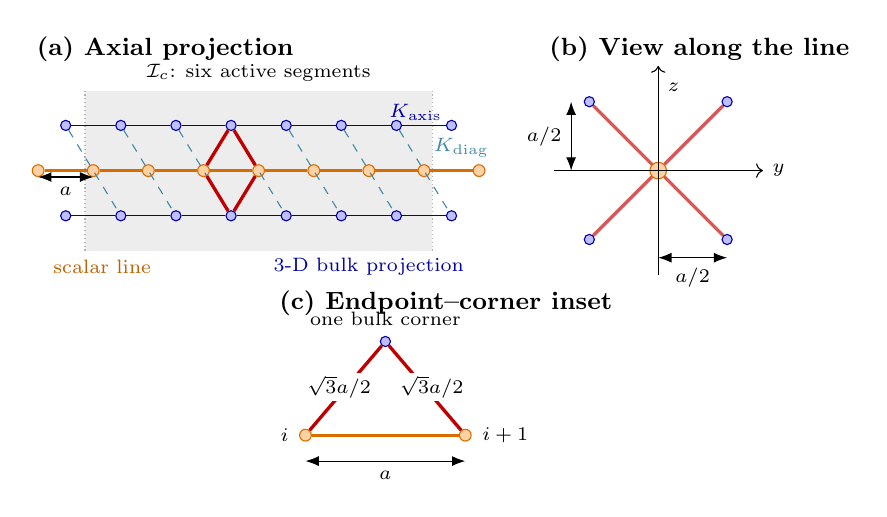
\begin{tikzpicture}[
    x=0.70cm,y=0.70cm,
    line/.style={draw=orange!85!black,very thick},
    linenode/.style={circle,draw=orange!85!black,fill=orange!35,inner sep=1.5pt},
    bulkbond/.style={draw=blue!65!black,thin},
    diagbond/.style={draw=cyan!65!black,thin,dashed},
    bulknode/.style={circle,draw=blue!65!black,fill=blue!25,inner sep=1.3pt},
    source/.style={draw=red!75!black,very thick},
    dim/.style={Latex-Latex,thin},
    lab/.style={font=\scriptsize},
    panel/.style={font=\bfseries\small}
]
% Panel A: axial projection
\begin{scope}[shift={(0,0)}]
  \node[panel,anchor=west] at (-0.2,2.20) {(a) Axial projection};
  \fill[gray!14] (0.85,-1.45) rectangle (7.15,1.45);
  \draw[gray!60,densely dotted] (0.85,-1.45) -- (0.85,1.45);
  \draw[gray!60,densely dotted] (7.15,-1.45) -- (7.15,1.45);
  \node[lab,anchor=south] at (4,1.45) {$\mathcal I_c$: six active segments};
  \foreach \i in {0,...,8}{\node[linenode] (q\i) at (\i,0) {};}
  \foreach \i in {0,...,7}{\draw[line] (q\i) -- (q\the\numexpr\i+1\relax);}
  \foreach \i in {0,...,7}{
    \node[bulknode] (bu\i) at (\i+0.5,0.82) {};
    \node[bulknode] (bd\i) at (\i+0.5,-0.82) {};
  }
  \foreach \i in {0,...,6}{
    \draw[bulkbond] (bu\i) -- (bu\the\numexpr\i+1\relax);
    \draw[bulkbond] (bd\i) -- (bd\the\numexpr\i+1\relax);
    \draw[diagbond] (bu\i) -- (bd\the\numexpr\i+1\relax);
  }
  \draw[source] (q3) -- (bu3);
  \draw[source] (q4) -- (bu3);
  \draw[source] (q3) -- (bd3);
  \draw[source] (q4) -- (bd3);
  \draw[dim] (q0.south) -- node[lab,below] {$a$} (q1.south);
  \node[lab,text=orange!75!black,anchor=west] at (0.1,-1.75) {scalar line};
  \node[lab,text=blue!65!black,anchor=east] at (7.9,-1.75) {3-D bulk projection};
  \node[lab,text=blue!65!black] at (6.85,1.06) {$K_{\rm axis}$};
  \node[lab,text=cyan!65!black] at (7.68,0.42) {$K_{\rm diag}$};
\end{scope}

% Panel B: transverse section
\begin{scope}[shift={(11.25,0)}]
  \node[panel,anchor=west] at (-2.15,2.20) {(b) View along the line};
  \node[linenode,minimum size=6pt] (c0) at (0,0) {};
  \foreach \yy/\zz in {1/1,1/-1,-1/1,-1/-1}{
    \node[bulknode] (c\yy\zz) at (1.25*\yy,1.25*\zz) {};
    \draw[source,opacity=0.65] (c0) -- (c\yy\zz);
  }
  \draw[->,thin] (-1.9,0) -- (1.9,0) node[right,lab] {$y$};
  \draw[->,thin] (0,-1.9) -- (0,1.9) node[pos=0.90,right,lab] {$z$};
  \draw[dim] (0,-1.58) -- node[lab,below] {$a/2$} (1.25,-1.58);
  \draw[dim] (-1.58,0) -- node[lab,left] {$a/2$} (-1.58,1.25);
\end{scope}

% Panel C: 3-D endpoint/corner inset, centered below
\begin{scope}[shift={(6.3,-4.35)}]
  \node[panel,anchor=west] at (-2.1,1.95) {(c) Endpoint--corner inset};
  \node[linenode] (L) at (-1.45,-0.45) {};
  \node[linenode] (R) at (1.45,-0.45) {};
  \node[bulknode] (C) at (0,1.25) {};
  \draw[line] (L) -- (R);
  \draw[source] (L) -- (C);
  \draw[source] (R) -- (C);
  \draw[dim] (-1.45,-0.92) -- node[lab,below] {$a$} (1.45,-0.92);
  \node[lab,fill=white,inner sep=1pt] at (-0.84,0.42) {$\sqrt3a/2$};
  \node[lab,fill=white,inner sep=1pt] at (0.84,0.42) {$\sqrt3a/2$};
  \node[lab,anchor=east] at (-1.58,-0.45) {$i$};
  \node[lab,anchor=west] at (1.58,-0.45) {$i+1$};
  \node[lab,anchor=south] at (0,1.36) {one bulk corner};
\end{scope}
\end{tikzpicture}%
}
\caption{Reference geometry in equilibrium lattice coordinates.  (a) Axial projection of the scalar line channel, one three-dimensional translated simple-cubic vector bulk, and the six-segment contact.  The source-link motif shown on one segment is repeated on every active segment.  Representative bulk axial and face-diagonal bonds are keyed by $K_{\rm axis}$ and $K_{\rm diag}$.  (b) View along the line. The four blue bulk sites lie in the segment's midpoint plane at $(y,z)=(s_y a/2,s_z a/2)$. The two line endpoints project onto the same orange mark. Each red radius shows the two springs joining those endpoints to one bulk site.  (c) Inset for one corner, showing endpoint separation $a$ and the two source-link rest lengths $\sqrt3a/2$.  Panel (a) is a projection of a single three-dimensional vector lattice, not a collection of independent planes.}
\label{fig:sectionII_geometry}
\end{figure*}

An internal observer uses calibrated clocks and spatial standards to register events in the lattice solution, such as a specified line site crossing equilibrium with positive axial velocity (SM6). For a common clock of constant rate $dt_{\rm id}/d\tau=F_0>0$ and the same energy standard, the incident and outgoing powers each scale by $1/F_0$. Their ratio is unchanged at the corresponding frequency $\omega_{\rm id}=\omega/F_0$.

\subsection{Quadratic central-force origin}
\label{sec:s2-harmonic-origin}

For a bulk bond or an active contact spring of family $\alpha$ with equilibrium vector $\vd=r_{0,\alpha}\hat{\vd}$, assume $V_\alpha\in C^3$ locally, $V_\alpha'(r_{0,\alpha})=0$, and $V_\alpha''(r_{0,\alpha})=\kappa_\alpha>0$. For $\Delta\vu=\vu_j-\vu_i$ with $|\Delta\vu|\ll r_{0,\alpha}$, the harmonic central-force reduction is~\cite{BornHuang1954,Maradudin1971}
\begin{equation}
  V_\alpha(|\vd+\Delta\vu|)-V_\alpha(r_{0,\alpha})
  =\frac{\kappa_\alpha}{2}(\hat{\vd}\cdot\Delta\vu)^2
  +\order(\Lambda_\alpha|\Delta\vu|^3),
  \label{eq:s2-energy-expansion}
\end{equation}
with finite local coefficient $\Lambda_\alpha$. We identify $\kappa_{\rm ax}=K_{\rm axis}$, $\kappa_{\rm fd}=K_{\rm diag}$, and $\kappa_{c,i}=g_i$. The quadratic bond energies are used exactly in the harmonic model. The local expansion is one possible mechanical origin, detailed in Supplementary Material Sec.~SM1, ``Harmonic origin.'' The scalar line is an effective one-dimensional harmonic channel and need not be the restriction of the same microscopic pair potential.

No onsite pinning term or externally prescribed transverse force is present. Transverse restoring forces in the bulk arise from the intersite vector central-force network, particularly the face-diagonal family.

\subsection{Complete canonical Hamiltonian}
\label{sec:s2-hamiltonian}

With overdots denoting $d/d\tau$, introduce canonical momenta
\begin{equation}
  p_i=m_q\dot q_i,
  \qquad
  \vp_{\bm r}=m_b\dot\vu_{\bm r}.
  \label{eq:s2-momenta}
\end{equation}
The Hamiltonian is
\begin{equation}
  H=H_q+H_b+H_c,
  \label{eq:s2-Htotal}
\end{equation}
where
\begin{equation}
  H_q
  =\sum_{i\in\mathbb Z}\frac{p_i^2}{2m_q}
  +\frac{K_q}{2}\sum_{i\in\mathbb Z}(q_{i+1}-q_i)^2,
  \label{eq:s2-Hq}
\end{equation}
\begin{align}
  H_b
  ={}&\sum_{\bm r\in\Lambdab}\frac{|\vp_{\bm r}|^2}{2m_b}
  \nonumber\\
  &+\frac12
  \sum_{\bm r\in\Lambdab}
  \sum_{\vd\in\mathcal D_{\rm ax}\cup\mathcal D_{\rm fd}}
  K_{\vd}
  \left[
  \hat{\vd}\cdot
  (\vu_{\bm r+\vd}-\vu_{\bm r})
  \right]^2,
  \label{eq:s2-Hb}
\end{align}
with $\Lambdab=\{\vR_{ijk}^{(b)}:i,j,k\in\mathbb Z\}$,
\begin{equation}
  K_{\vd}=
  \begin{cases}
    K_{\rm axis},&\vd\in\mathcal D_{\rm ax},\\
    K_{\rm diag},&\vd\in\mathcal D_{\rm fd},
  \end{cases}
  \qquad
  \hat{\vd}=\vd/|\vd|.
  \label{eq:s2-Kd}
\end{equation}
The positive representatives in Eqs.~\eqref{eq:s2-Dax}--\eqref{eq:s2-Dfd} count each undirected bulk bond once; the factor $1/2$ in Eq.~\eqref{eq:s2-Hb} is the physical spring-energy coefficient.

For one corner, write $\vu=\vu_{i,s_y,s_z}^{(c)}$ and define the equilibrium source-link directions
\begin{equation}
  \hat{\bm n}_L=\frac{(1,s_y,s_z)}{\sqrt3},
  \qquad
  \hat{\bm n}_R=\frac{(-1,s_y,s_z)}{\sqrt3}.
  \label{eq:s2-source-directions}
\end{equation}
The two physical links attached to that corner contribute
\begin{align}
  H_{c,i}^{(s_y,s_z)}
  ={}&\frac{g_i}{2}
  \left[
  \hat{\bm n}_L\cdot(\vu-q_i\ex)
  \right]^2
  \nonumber\\
  &+\frac{g_i}{2}
  \left[
  \hat{\bm n}_R\cdot(\vu-q_{i+1}\ex)
  \right]^2,
  \label{eq:s2-Hc-corner}
\end{align}
and the complete finite coupling Hamiltonian is
\begin{equation}
  H_c
  =\sum_{i\in\Ic}
   \sum_{s_y=\pm1}
   \sum_{s_z=\pm1}
   H_{c,i}^{(s_y,s_z)}.
  \label{eq:s2-Hc-total}
\end{equation}
With
\begin{equation}
  \bar q_i=\frac{q_i+q_{i+1}}{2},
  \qquad
  \Delta q_i=q_{i+1}-q_i,
  \label{eq:s2-qbar-delta}
\end{equation}
Eq.~\eqref{eq:s2-Hc-corner} reduces identically to
\begin{equation}
  H_{c,i}^{(s_y,s_z)}
  =\frac{g_i}{3}
  \left[
  (u_x-\bar q_i)^2
  +\left(
  s_yu_y+s_zu_z+\frac{\Delta q_i}{2}
  \right)^2
  \right].
  \label{eq:s2-Hc-reduced}
\end{equation}
The mean endpoint displacement $\bar q_i$ couples to the corner's axial motion $u_x$. The endpoint displacement difference $\Delta q_i$ couples to the signed transverse combination $s_yu_y+s_zu_z$. The two squares follow by an algebraic rotation of the physical spring extensions. Each square contributes to the local spring energy. The bulk dynamical matrix separately determines the modal polarizations.

We assume
\begin{equation}
\begin{gathered}
  m_q,m_b,K_q,K_{\rm axis},K_{\rm diag}>0,\\
  g_i\ge0.
\end{gathered}
\label{eq:s2-positivity}
\end{equation}
The mass matrix is positive definite and the potential-energy stiffness matrix is real symmetric and positive semidefinite, hence $H\ge0$. Because $H$ has no explicit $\tau$ dependence, unforced Hamiltonian evolution conserves $H$; the model contains no gain, gyroscopic term, or velocity-dependent coupling. The underlying equations are therefore time-reversal invariant and reciprocal. The scattering formulation expresses this reciprocity for flux-normalized channels in Eq.~\eqref{eq:reciprocity}.

The infinite sums in Eqs.~\eqref{eq:s2-Hq}--\eqref{eq:s2-Hc-total} are first understood on finite-energy configurations or finite volumes. Bloch and scattering states use per-cell or unit-flux normalization, followed by the standard infinite-volume scattering limit~\cite{Ong2018,Sadasivam2017,Khodavirdi2024}.

\subsection{Reference units, equilibrium, and nullspaces}
\label{sec:s2-units-nullspaces}

Take $a$, $m_b$, and $K_{\rm diag}$ as reference units. The dimensionless reference ratios are
\begin{equation}
  \frac{m_q}{m_b}=1,
  \qquad
  \frac{K_{\rm axis}}{K_{\rm diag}}=1,
  \qquad
  \frac{K_q}{K_{\rm diag}}=1.69,
  \label{eq:s2-ratios}
\end{equation}
with the symmetric six-segment reference taper
\begin{equation}
  \frac{(g_{i_0},g_{i_0+1},\ldots,g_{i_0+5})}{K_{\rm diag}}
  =(0.1,0.2,0.2,0.2,0.2,0.1).
  \label{eq:s2-g-profile}
\end{equation}
The reference assigns equal masses to the line and bulk sites. Equal axial and diagonal bulk stiffnesses give an isotropic long-wavelength acoustic limit (Sec.~\ref{sec:s4-bulk-spectrum}). With these masses, $K_q/K_{\rm diag}=1.69$ places the long-wavelength line speed between the bulk shear and longitudinal speeds. In units of $a\sqrt{K_{\rm diag}/m_b}$, the three speeds are $c_T=1$, $c_q=1.3$ and $c_L=\sqrt{3}$ (Eqs.~\eqref{eq:s2-line-speed} and \eqref{eq:s4-acoustic-speeds}). Dimensional units may be restored using
\begin{equation}
  [q]=[u]=a,
  \qquad
  [\tau]=\sqrt{m_b/K_{\rm diag}},
  \qquad
  [E]=K_{\rm diag}a^2.
  \label{eq:s2-units}
\end{equation}
Numerical frequencies below are conjugate to $\tau$ and, unless stated otherwise, are quoted in units of $\sqrt{K_{\rm diag}/m_b}$. Thus $\omega=1.2$ means $\omega\sqrt{m_b/K_{\rm diag}}=1.2$.

For the reference taper at $\omega=1.2$, $c_q=1.3$ gave the largest incident-to-qT conversion among ten line speeds tested by varying $K_q$ at fixed masses. The stiffness sweep in Sec.~\ref{sec:s9-robustness} retains the units of the unvaried reference system while $K_{\rm diag}$ changes. Wavevectors refer to the equilibrium lattice coordinates, retain inverse-length units, and enter through dimensionless products such as $\vk a$. The speeds $c_q$, $c_T$, $c_L$, and the group velocities below are propagation rates per unit $\tau$ in these coordinates.

At $q_i=0$ and $\vu_{ijk}=0$, every bond is at its rest length and all first derivatives of the potential vanish. The uncoupled line dispersion is
\begin{equation}
  \omega_q^2(k_x)
  =\frac{4K_q}{m_q}
   \sin^2\!\left(\frac{k_xa}{2}\right),
  \label{eq:s2-line-dispersion}
\end{equation}
with long-wave line speed
\begin{equation}
  c_q=\lim_{k_x\to0^+}\frac{\omega_q(k_x)}{k_x}
  =a\sqrt{\frac{K_q}{m_q}}.
  \label{eq:s2-line-speed}
\end{equation}
The line's only zero frequency in the first Brillouin zone occurs at $k_x=0$ (uniform axial motion). For $K_{\rm axis},K_{\rm diag}>0$, the infinite bulk's only Bloch zero modes are the three uniform translations at $\vk=0$ (Sec.~\ref{sec:s4-bulk-spectrum}).

A free finite truncation of the lattice has rigid-body motions and may admit other zero-energy motions. For an infinitesimally rigid finite bulk, a connected line and at least one complete positive motif, the nullspace of the combined free line-and-bulk truncation is spanned by common axial translation and rigid bulk rotation about the line (SM1, ``Finite fixtures and conditional kernel''). SM1 reports tests on such truncations, and the validation archive (see the Data Availability Statement) records which bonds each truncation includes. The scattering calculations use positive frequencies.



\section{Local paired-link generation mechanism}
\label{sec:s3-mechanism}

At each active segment of the contact in Fig.~\ref{fig:sectionII_geometry}, a pair of inclined springs joins each of the four surrounding corners to the two segment endpoints [Fig.~\ref{fig:s3-mechanism}(a)]. As a longitudinal wave passes, axial displacement of the segment midpoint contributes an axial force on the corner, and a change in endpoint separation contributes a radial force. The total contact force also depends on the corner displacement. We derive these contributions from the spring energy~\cite{BornHuang1954,Maradudin1971} and then sum the radial forces over the four corners.

The signs $c=(s_y,s_z)$ identify a corner. Its outward direction in the equilibrium transverse plane is given by
\begin{align}
  \Cc&=\{(s_y,s_z):s_y,s_z=\pm1\},\\
  \vt_c&=s_y\ey+s_z\ez.
  \label{eq:s3-corners}
\end{align}
The vector has length $|\vt_c|=\sqrt2$. For corner displacement $\vu_{ic}$, define
\begin{equation}
  \bar q_i=\frac{q_i+q_{i+1}}{2},
  \quad
  \Delta q_i=q_{i+1}-q_i,
  \quad
  S_{ic}=\vt_c\!\cdot\vu_{ic},
  \label{eq:s3-kinematic-defs}
\end{equation}
\begin{equation}
  A_{ic}=u_{ic,x}-\bar q_i,
  \qquad
  B_{ic}=S_{ic}+\frac{\Delta q_i}{2}.
  \label{eq:s3-AB}
\end{equation}
Here $S_{ic}$ is $\sqrt2$ times the signed corner displacement along the outward radial unit vector $\vt_c/\sqrt2$. The coordinate $A_{ic}$ measures axial displacement relative to the endpoint mean, while $B_{ic}$ combines $S_{ic}$ with half the segment extension. The two springs store the harmonic energy
\begin{equation}
  H_{c,ic}=\frac{g_i}{3}\left(A_{ic}^{2}+B_{ic}^{2}\right).
  \label{eq:s3-Hcorner}
\end{equation}
The length change $\Delta q_i$ is positive for extension and negative for compression. The dimensionless segment strain is $\Delta q_i/a$. Supplementary Material Sec.~SM1, ``Source coordinates and optional inverse-spacing dictionary,'' gives the reciprocal segment length $1/(a+\Delta q_i)$ for $a+\Delta q_i>0$ and states the limits of this kinematic interpretation.

\subsection{Exact forces and line-driven source terms}
\label{sec:s3-forces}

Taking the negative derivatives of the spring energy with respect to the corner displacement and the two endpoint displacements gives
\begin{align}
  \vF_{b,ic}
  &=-\frac{2g_i}{3}
  \left(A_{ic}\ex+B_{ic}\vt_c\right),
  \label{eq:s3-corner-force}\\
  Q_{i\leftarrow c}
  &=-\frac{\partial H_{c,ic}}{\partial q_i}
   =\frac{g_i}{3}(A_{ic}+B_{ic}),
  \label{eq:s3-left-generalized-force}\\
  Q_{i+1\leftarrow c}
  &=-\frac{\partial H_{c,ic}}{\partial q_{i+1}}
   =\frac{g_i}{3}(A_{ic}-B_{ic}).
  \label{eq:s3-right-generalized-force}
\end{align}
The scalar line coordinates give the axial endpoint reactions $Q_{i\leftarrow c}$ and $Q_{i+1\leftarrow c}$. A common axial translation of both endpoints and the corner leaves the spring energy unchanged, so the sum of the reactions balances the axial force on the corner,
\begin{equation}
  \ex\!\cdot\vF_{b,ic}
  +Q_{i\leftarrow c}+Q_{i+1\leftarrow c}=0.
  \label{eq:s3-axial-reciprocity}
\end{equation}
Reciprocity follows from equality of the mixed line--corner derivatives of the energy. The corner force contains a restoring term and two terms driven by the line, the axial-average source $X$ and the radial source $R$,
\begin{equation}
  \vF_{b,ic}
  =-\frac{2g_i}{3}
  \left(u_{ic,x}\ex+S_{ic}\vt_c\right)
  +\underbrace{\frac{2g_i}{3}\bar q_i\ex}_{\vF^{\rm src}_{X,ic}}
  +\underbrace{-\frac{g_i}{3}\Delta q_i\vt_c}_{\vF^{\rm src}_{R,ic}}.
  \label{eq:s3-source-split}
\end{equation}
At the corner's reference position, $\vu_{ic}=0$, the restoring term vanishes. The transverse components of the contact force are then
\begin{equation}
  F_y=-\frac{g_i}{3}s_y\Delta q_i,
  \qquad
  F_z=-\frac{g_i}{3}s_z\Delta q_i.
  \label{eq:s3-initial-transverse-force}
\end{equation}
To isolate the radial contribution, hold the corner at its reference position and extend an active segment about a fixed midpoint. Both springs lengthen. Their axial forces on the corner cancel, while their transverse forces add and pull the corner toward the line [Fig.~\ref{fig:s3-mechanism}(b)]. Compression reverses these forces and pushes the corner outward. If both endpoints and the corner translate together axially from equilibrium, both springs remain unloaded, and the axial source and restoring terms in Eq.~\eqref{eq:s3-source-split} cancel. In scattering, the line and bulk respond to their mutual forces without an imposed transverse drive.

\begin{figure*}[!t]
\centering
\resizebox{0.98\textwidth}{!}{%
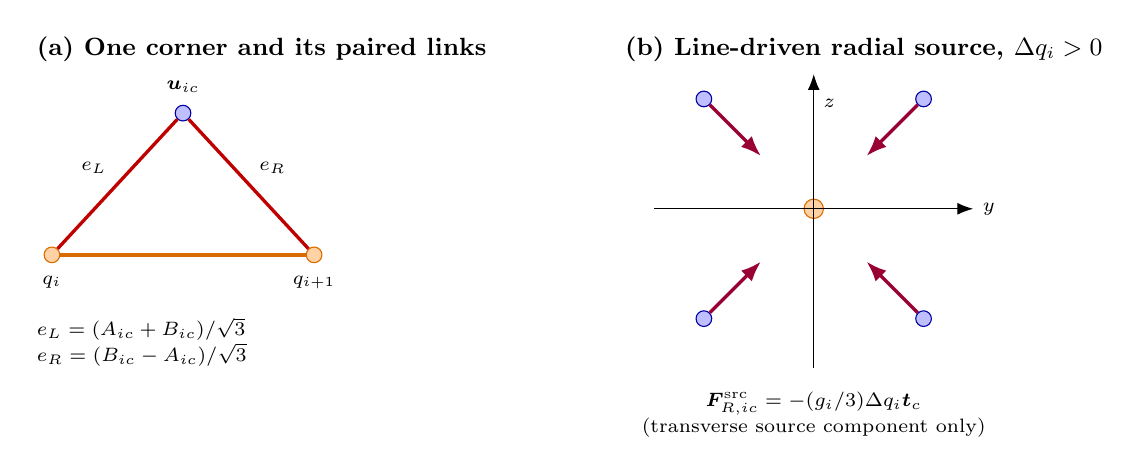
\begin{tikzpicture}[
  x=0.90cm,y=0.90cm,
  linenode/.style={circle,draw=orange!85!black,fill=orange!35,inner sep=2.0pt},
  bulknode/.style={circle,draw=blue!65!black,fill=blue!25,inner sep=2.0pt},
  spring/.style={draw=red!75!black,very thick},
  force/.style={-{Latex[length=2.6mm]},draw=purple!80!black,very thick},
  axis/.style={-{Latex[length=2.0mm]},thin},
  lab/.style={font=\scriptsize},
  panel/.style={font=\bfseries\small}
]
% Panel A
\begin{scope}[shift={(0,0)}]
  \node[panel,anchor=west] at (-2.2,2.25) {(a) One corner and its paired links};
  \node[linenode] (L) at (-1.85,-0.65) {};
  \node[linenode] (R) at (1.85,-0.65) {};
  \node[bulknode] (C) at (0,1.35) {};
  \draw[orange!85!black,very thick] (L)--(R);
  \draw[spring] (L)--node[lab,above left] {$e_L$}(C);
  \draw[spring] (R)--node[lab,above right] {$e_R$}(C);
  \node[lab,below=1pt of L] {$q_i$};
  \node[lab,below=1pt of R] {$q_{i+1}$};
  \node[lab,above=1pt of C] {$\vu_{ic}$};
  \node[lab,align=left,anchor=north west] at (-2.2,-1.40)
    {$e_L=(A_{ic}+B_{ic})/\sqrt3$\\$e_R=(B_{ic}-A_{ic})/\sqrt3$};
\end{scope}
% Panel B
\begin{scope}[shift={(8.9,0)}]
  \node[panel,anchor=west] at (-2.8,2.25) {(b) Line-driven radial source, $\Delta q_i>0$};
  \node[linenode,minimum size=7pt] (O) at (0,0) {};
  \foreach \yy/\zz in {1/1,1/-1,-1/1,-1/-1}{
    \node[bulknode] (B\yy\zz) at (1.55*\yy,1.55*\zz) {};
    \draw[force] (B\yy\zz) -- ($(B\yy\zz)!0.52!(O)$);
  }
  \draw[axis] (-2.25,0)--(2.25,0) node[right,lab] {$y$};
  \draw[axis] (0,-2.25)--(0,1.90) node[pos=0.90,right,lab] {$z$};
  \node[lab,align=center,anchor=north] at (0,-2.45)
    {$\vF^{\rm src}_{R,ic}=-(g_i/3)\Delta q_i\vt_c$\\(transverse source component only)};
\end{scope}
\end{tikzpicture}%
}
\caption{Paired-link forces in equilibrium lattice coordinates. (a) The two springs join one corner to the line endpoints. The difference $e_L-e_R$ and sum $e_L+e_R$ of their signed harmonic extensions are proportional to the deformation coordinates $A_{ic}$ and $B_{ic}$, respectively. (b) Viewed along the line, the endpoints project onto the orange center. Arrows show the radial source $\vF^{\rm src}_{R,ic}$ at $(y,z)=(s_y a/2,s_z a/2)$ for extension. They reverse for compression. The full corner force also includes the axial source and restoring term. Equations~\eqref{eq:s3-radial-resultant}--\eqref{eq:s3-radial-dipole} give the radial resultant, torque and first moment.}
\label{fig:s3-mechanism}
\end{figure*}

\subsection{Radial force moment and finite-contact Fourier transform}
\label{sec:s3-dipole-fourier}

Measured from the segment midpoint, each equilibrium corner has position
\begin{equation}
  \vrr_c=\frac{a}{2}\vt_c,
  \label{eq:s3-corner-radius}
\end{equation}
and its radial source force $\vF^{\rm src}_{R,ic}$ is collinear with this position. Each radial torque therefore vanishes. The forces at opposite corners cancel in pairs, giving
\begin{align}
  \sum_{c\in\Cc}\vF^{\rm src}_{R,ic}&=0,\label{eq:s3-radial-resultant}\\
  \sum_{c\in\Cc}\vrr_c\times\vF^{\rm src}_{R,ic}&=0.
  \label{eq:s3-radial-balance}
\end{align}
The first spatial moment distinguishes inward from outward forces even when their resultant vanishes. In the elastodynamic convention
\begin{equation}
  M^R_{\alpha\beta}
  =\sum_{c\in\Cc}F^{\rm src}_{R,ic,\alpha}r_{c,\beta},
  \label{eq:s3-moment-definition}
\end{equation}
for a balanced force system~\cite{AkiRichards2002}, the four corner contributions give
\begin{equation}
  \bm M_i^R
  =-\frac{2g_i a\Delta q_i}{3}
  \operatorname{diag}(0,1,1).
  \label{eq:s3-radial-dipole}
\end{equation}
The four equivalent spring pairs cancel the radial resultant on each segment separately, even when their common stiffness $g_i$ varies from segment to segment. For $g_i\Delta q_i\ne0$ the resulting symmetric transverse force dipole is contractile in extension and extensile in compression. Its trace, $-4g_i a\Delta q_i/3$, gives a nonzero isotropic part alongside the deviatoric part. If $g_i=0$ or $\Delta q_i=0$, the radial source and its moment vanish.

The spatial Fourier transform weights each force by its phase $e^{-i\vk\cdot\vrr}$. For one segment at fixed extension, the constant term vanishes with the radial resultant. The first spatial moment therefore gives the term linear in $\vk$ at long wavelengths. At frequency $\omega$, let $Q_i^{\rm full}$ be the displacement amplitude at line site $i$ including the reaction from the bulk,
\begin{align}
 q_i(\tau)&=\operatorname{Re}\!\left[Q_i^{\rm full}(\omega)e^{-i\omega\tau}\right],\\
 \Delta Q_i^{\rm full}(\omega)&=Q_{i+1}^{\rm full}(\omega)-Q_i^{\rm full}(\omega).
 \label{eq:s3-fixed-frequency-phasor}
\end{align}
Summing over the corners and then along the finite contact gives the line-driven radial source transform
\begin{align}
  \widetilde{\vF}^{\rm slab}_{R}(\vk;\omega)
  &=\frac{4i}{3}\,\bm s_\perp(\vk)
  \sum_{i\in\Ic}g_i\Delta Q_i^{\rm full}(\omega)
  e^{-ik_x(i+1/2)a},\\
  \bm s_\perp(\vk)
  &=\begin{pmatrix}
    0\\
    \sin(k_ya/2)\cos(k_za/2)\\
    \cos(k_ya/2)\sin(k_za/2)
  \end{pmatrix}.
  \label{eq:s3-general-slab-source}
\end{align}
The subscript $\perp$ in $\bm s_\perp$ refers to the line axis. For a bulk wavevector along the line ($k_y=k_z=0$), the four corners of each segment have identical phase factors, so each segment contributes zero radial Fourier amplitude. For other directions the phases can differ. When $k_z=0$, $\bm s_\perp=\sin(k_y a/2)\ey$. For a wavevector along $y$, this factor can thus be nonzero and parallel to the wavevector, with zero projection onto shear polarizations in the isotropic long-wavelength limit.

The finite axial sum weights each actual segment extension by $g_i$ and permits unequal incident and outgoing axial wave numbers. Outgoing power depends on how the full force response projects onto propagating bulk modes. Supplementary Material Sec.~SM1, ``Source transforms and prescribed-Bloch asymptotics,'' gives the local transform, the finite-contact phase sum for a prescribed Bloch wave on the line, and the long-wavelength expansion of the prescribed source. Section~\ref{pred:sec-lowfreq} derives the low-frequency radiation law with the line responding to the bulk.

\subsection{Contact work and transverse reactions on the line}
\label{sec:s3-XR-work}

To track work on the line and bulk, split the per-corner energy into its two terms,
\begin{equation}
  H_{X,ic}=\frac{g_i}{3}A_{ic}^2,
  \qquad
  H_{R,ic}=\frac{g_i}{3}B_{ic}^2.
  \label{eq:s3-XR-energies}
\end{equation}
In terms of the signed harmonic extensions $e_L$ and $e_R$ of the left and right springs in Fig.~\ref{fig:s3-mechanism}(a),
\begin{equation}
  H_{X,ic}=\frac{g_i}{4}(e_L-e_R)^2,
  \qquad
  H_{R,ic}=\frac{g_i}{4}(e_L+e_R)^2.
  \label{eq:s3-XR-physical-springs}
\end{equation}
The corresponding complete coupling sectors are
\begin{equation}
\begin{aligned}
 H_X&=\sum_{i\in\Ic}\sum_{c\in\Cc}H_{X,ic},\\
 H_R&=\sum_{i\in\Ic}\sum_{c\in\Cc}H_{R,ic},\\
 H_c&=H_X+H_R.
\end{aligned}
 \label{eq:s3-XR-global}
\end{equation}
Thus $X$ and $R$ combine the extensions of the same two springs. The $y$ and $z$ displacements enter the single radial combination $s_yu_y+s_zu_z$. These local variables do not specify two bulk eigenbranches or two independently controlled polarizations.

For time-independent $g_i$, the powers delivered to the line and bulk by each term sum to the rate at which it loses stored spring energy. Storage explains why the instantaneous powers can differ in magnitude. The total contact work is the sum of the $X$ and $R$ contributions, as shown in Supplementary Material Sec.~SM1, ``$X/R$ component powers and storage''.

The bulk fields from $X$ and $R$ can interfere in the coupled solution. Keeping only $H_X$ or only $H_R$ changes the stiffness and hence the motion, so the separately calculated transmissions need not add to the full transmission (Sec.~\ref{sec:s6-controls}).

The scalar line admits only axial motion. To check for transverse endpoint reactions under axial line excitation, temporarily give each endpoint three displacement coordinates. Evaluate the spring forces on the centered response that is invariant under the rotations and reflections of the square of corners (the $A_1$ sector of $C_{4v}$),
\begin{equation}
  \vu_{ic}=U_{X,i}\ex+U_{R,i}\vt_c,
  \label{eq:s3-A1-state}
\end{equation}
where $U_{R,i}$ multiplies the unnormalized $\vt_c$. Then $S_{ic}=2U_{R,i}$, so $A_{ic}$ and $B_{ic}$ have the same values at all four corners. The transverse force on each embedded endpoint is proportional to
\begin{equation}
  \sum_{c\in\Cc}\vt_c=0,
  \label{eq:s3-sign-sum}
\end{equation}
so
\begin{equation}
  \vF^{\rm emb}_{q_i,\perp}
  =\vF^{\rm emb}_{q_{i+1},\perp}=0.
  \label{eq:s3-embedded-reaction}
\end{equation}
On this symmetric state the net transverse force vanishes at each endpoint even in the vector-coordinate calculation. Hence the transverse endpoint reactions do no work. The complete $R$ force at each corner is a common coefficient times $\vt_c$. Its resultant and each radial torque vanish. The $X$ force is common and axial. Its total torque vanishes because $\sum_c\vrr_c=0$, and the endpoint reactions balance its resultant by Eq.~\eqref{eq:s3-axial-reciprocity}. This closes the force and torque balance on the centered state. Away from this symmetry, transverse endpoint reactions can occur.

Here radial denotes the direction from the line axis to a corner in the transverse plane. In the isotropic acoustic limit, shear polarization is perpendicular to the wavevector, so even an axial force can excite shear in oblique directions.

\section{Three-dimensional bulk modes and exact source symmetry}
\label{sec:s4-bulk-symmetry}

To calculate the outgoing power, we need the bulk polarizations at the drive frequency and the corner displacement patterns accessible to the centered line. The construction follows harmonic-lattice and point-group methods~\cite{BornHuang1954,Maradudin1971,Dresselhaus2008}.

\subsection{Bulk spectrum and the quasi-transverse pair}
\label{sec:s4-bulk-spectrum}

The phase of a Bloch wave varies across sites. Its polarization $\ve_\lambda$ gives the relative amplitudes and phases of the three displacement components at every site. In the displacement units of Sec.~\ref{sec:s2-model}, the unit-amplitude mode is
\begin{equation}
  \vu_{\vR}(\tau)
  =\operatorname{Re}\!\left[
    \ve_\lambda(\vk)
    e^{i(\vk\cdot\vR-\omega_\lambda\tau)}
  \right],
  \qquad
  \ve_\lambda^\dagger\ve_\mu=\delta_{\lambda\mu},
  \label{eq:s4-bloch-convention}
\end{equation}
where $\omega_\lambda$ is the angular frequency with respect to time $\tau$. The three eigenvalues of the mass-normalized dynamical matrix $D(\vk)$ are the squared frequencies,
\begin{equation}
  D(\vk)\ve_\lambda(\vk)
  =\omega_\lambda^2(\vk)\ve_\lambda(\vk),
  \qquad
  -\frac{\pi}{a}\leq k_\alpha<\frac{\pi}{a}.
  \label{eq:s4-eigenproblem}
\end{equation}
Each spring responds to displacement along its bond. Summing one representative of each undirected axial and face-diagonal bond from Sec.~\ref{sec:s2-model} gives
\begin{equation}
  D(\vk)
  =\frac{2}{m_b}
   \sum_{\bm d\in\mathcal D_{\rm ax}\cup\mathcal D_{\rm fd}}
   K_{\bm d}
   \left[1-\cos(\vk\cdot\bm d)\right]
   \hat{\bm d}\hat{\bm d}^{\mathsf T}.
  \label{eq:s4-dynamical-matrix}
\end{equation}
The factor follows from
$2-e^{i\vk\cdot\bm d}-e^{-i\vk\cdot\bm d}
 =2[1-\cos(\vk\cdot\bm d)]$.
For $K_{\rm axis},K_{\rm diag}>0$, every term is positive semidefinite. At $\vk=0$, the three rigid translations have zero frequency. For $\vk\ne0$ in the first Brillouin zone, choose an axis $i$ with $k_i\ne0$. A displacement with zero frequency must have zero component along every such axis, by the axial springs. For any remaining axis $j$ with $k_j=0$, a face diagonal in the $ij$ plane has a nonzero phase difference and forces the $j$ component to vanish. Hence
\begin{equation}
  \ker D(\vk)=\{0\},
  \qquad \vk\neq0.
  \label{eq:s4-rigidity}
\end{equation}
Along a coordinate axis, purely axial springs would leave transverse displacements with no restoring force. The face diagonals supply that force.

To identify shear and longitudinal motion, take the wavelength large compared with the lattice spacing $a$. For the reference choice $K_{\rm axis}=K_{\rm diag}=K$, the long-wave expansion is
\begin{equation}
  D(\vk)
  =\frac{Ka^2}{m_b}
   \left(|\vk|^2 I+2\vk\vk^{\mathsf T}\right)
   +\order\!\left(\frac{Ka^4}{m_b}|\vk|^4\right),
  \label{eq:s4-long-wave}
\end{equation}
where the operator-norm remainder bounds the error for every unit displacement polarization. The leading eigenvalue for either polarization perpendicular to $\vk$ is $Ka^2|\vk|^2/m_b$. Along $\vk$ it is three times as large. The shear and longitudinal sound speeds are
\begin{equation}
  c_T=a\sqrt{K/m_b},
  \qquad
  c_L=\sqrt3\,c_T.
  \label{eq:s4-acoustic-speeds}
\end{equation}
These leading speeds are independent of direction. At finite spacing the spectrum retains cubic anisotropy. For general bond stiffnesses the continuum elastic constants are
\begin{equation}
\begin{aligned}
 C_{11}&=(K_{\rm axis}+2K_{\rm diag})/a,\\
 C_{12}&=C_{44}=K_{\rm diag}/a.
\end{aligned}
\label{eq:s4-cauchy-constants}
\end{equation}
Thus $K_{\rm axis}=K_{\rm diag}=K$ selects an isotropic Cauchy solid with Lam\'e constants $\lambda=\mu=K/a$ and Poisson ratio $1/4$. With continuum mass density $m_b/a^3$, this recovers Eq.~\eqref{eq:s4-acoustic-speeds}. Unequal stiffnesses generally give a cubic-anisotropic continuum.

Figure~\ref{fig:s4-bulk-symmetry}(a) compares the bulk branches at one axial wave number, the incident value $\kappa_q$. Label the branches $0,1,2$ in order of increasing squared frequency, allowing ties. At the reference frequency $\omega=1.2$, the right-moving line wave in Eq.~\eqref{eq:s2-line-dispersion} has
\begin{align}
  \kappa_q
  &=\frac{2}{a}\arcsin\!\left[
    \frac{\omega}{2}\sqrt{\frac{m_q}{K_q}}
  \right],\\
  \kappa_q a&\simeq0.95946,\\
  \lambda_q&\equiv2\pi/\kappa_q,
  &\lambda_q/a\simeq6.5487.
  \label{eq:s4-line-carrier}
\end{align}
At $k_x=\kappa_q$, each lower branch has regular points at $\omega=1.2$ in the transverse zone. The upper branch has a higher minimum on this slice,
\begin{equation}
  \omega_{2,\min}(k_x=\kappa_q)\simeq1.598816.
  \label{eq:s4-upper-threshold}
\end{equation}
Equation~\eqref{eq:s4-dynamical-matrix} gives $(m_b/K)D_{xx}=6-2\cos(\kappa_q a)[1+\cos(k_y a)+\cos(k_z a)]$. Since $\cos(\kappa_q a)>0$, $D_{xx}$ is smallest at $k_y=k_z=0$. The largest eigenvalue is bounded below by $D_{xx}$ and equals it there. The square root gives Eq.~\eqref{eq:s4-upper-threshold}, confirming the transverse-zone search. The finite contact permits other axial wave numbers (see the prescribed-wave phase sum in Supplementary Material Sec.~SM1). On the bulk axis the upper branch reaches the drive at $k_xa\simeq0.70748$. Section~\ref{sec:s5-scattering} calculates the branch powers with the line and bulk coupled.

\begin{figure*}[!t]
  \centering
  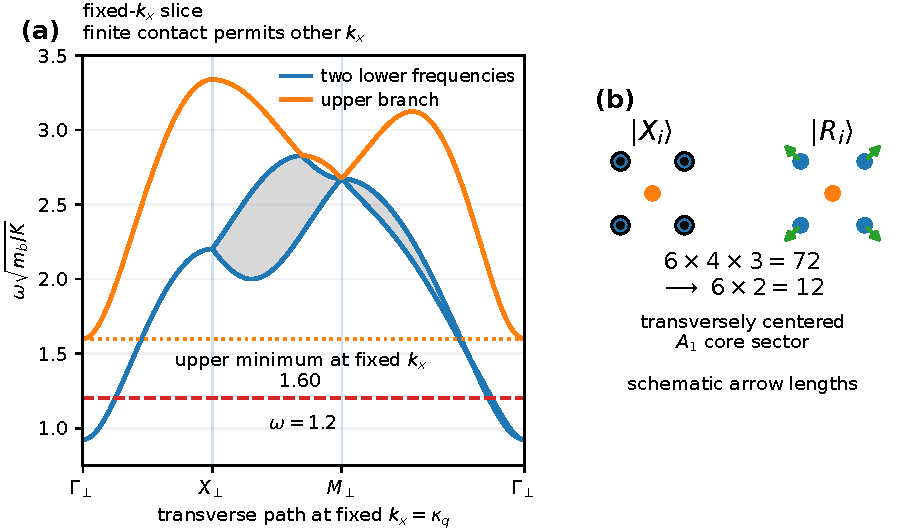
\includegraphics[width=0.98\textwidth]{figures/paper1_sectionIV_fig3_bulk_modes_symmetry_v2.pdf}
  \caption{Bulk modes and contact symmetry in equilibrium lattice coordinates. (a) Exact bulk frequencies, conjugate to $\tau$, along $\Gamma_\perp(0,0)\to X_\perp(\pi/a,0)\to M_\perp(\pi/a,\pi/a)\to\Gamma_\perp(0,0)$ at $k_x=\kappa_q$. The blue curves coincide on $\Gamma_\perp X_\perp$ and cross the drive frequency $\omega=1.2$ (dashed line) separately on $M_\perp\Gamma_\perp$. Shading marks the interval between them. All three branches meet above the drive at $M_\perp$. The dotted line marks the upper minimum on this slice. The crossings locate resonant modes. SM2 gives a nonzero source overlap on each lower branch at wavevectors off this slice. (b) Axial corner displacements are shown end-on, and arrows show the outward radial basis pattern. Segment $i$ has local index $s$, with $i=i_0+s-1$. Arrow lengths are schematic. The coupled motion sets the amplitudes. Two normalized patterns per segment represent the centered response of the 72 corner coordinates with 12 amplitudes.}
  \label{fig:s4-bulk-symmetry}
\end{figure*}

The frequency shell of branch $\lambda$ contains the bulk wavevectors at which it oscillates at the drive frequency,
\begin{equation}
  \Sigma_\lambda(\omega)
  =\{\vk\in\BZ:\omega_\lambda(\vk)=\omega\},
  \label{eq:s4-branch-shell}
\end{equation}
where $\BZ$ is the first Brillouin zone. On an operating set $\Omega_{\rm op}\subset\BZ\setminus\{0\}$ where $\omega_2^2-\omega_1^2$ stays bounded away from zero, the upper polarization spans a line and the lower two span its orthogonal plane. We group the branches into two polarization clusters, the quasi-longitudinal (qL) upper branch and the quasi-transverse (qT) lower pair, with projectors
\begin{equation}
  \PqL(\vk)=\ve_2\ve_2^\dagger,
  \qquad
  \PqT(\vk)=I-\PqL(\vk).
  \label{eq:s4-cluster-projectors}
\end{equation}
At each $\vk$ the corner forces add with Bloch phases $e^{-i\vk\cdot\vR_r}$ set by their equilibrium positions $\vR_r$ (Sec.~\ref{sec:s3-mechanism}). The projector $\PqT(\vk)$ maps this three-component Fourier force onto the lower plane independently of the basis. At a lower-mode degeneracy any orthonormal basis of the plane gives eigenmodes. A basis rotation generally mixes modes with distinct frequencies. Equation~\eqref{eq:s5-cluster-spectral} selects modes at the drive frequency with weights $\delta(\omega_\lambda^2-\omega^2)$. The matrix of these mode weights is diagonal in the eigenmode basis and can have off-diagonal entries in a rotated basis of the lower plane.

How nearly transverse is this plane? Among its unit displacement vectors, the largest squared component along the wave normal $\hat{\vk}$ is
\begin{equation}
  \ell_{\rm qT}^{(k)}(\vk)
  =\hat{\vk}^{\dagger}\PqT(\vk)\hat{\vk},
  \qquad \hat{\vk}=\vk/|\vk|.
  \label{eq:s4-cluster-leakage}
\end{equation}
For $K_{\rm axis}=K_{\rm diag}=K$ and $0<\rho=a|\vk|<2$, the gap above the lower pair is positive at each wavevector and tends to zero at the origin. The nine bond families give
\[
 \|P_{\qT}(\vk)\hat{\vk}\|\leq\frac{\rho^2}{4},
 \qquad
 \ell_{\rm qT}^{(k)}(\vk)\leq\frac{\rho^4}{16}.
\]
The proof in Supplementary Material Sec.~SM2, under \emph{A sufficient acoustic polarization bound}, also covers a degeneracy within the lower pair. The bound concerns the displacement of a homogeneous bulk mode relative to its wave normal. The direction of energy flow and the fraction of incident power converted require separate calculations.

At $\omega=1.2$, SM2 proves that the upper branch is separated from the lower pair on every resonant shell by at least $0.8448$ in squared-frequency units, and that each simple resonant branch has nonzero group speed. A numerical search, with each candidate refined back onto its shell, gives
\begin{align}
  \min_{\Sigma_0\cup\Sigma_1\cup\Sigma_2}
  (\omega_2^2-\omega_1^2)&\simeq0.9391,\\
  \max_{\Sigma_0\cup\Sigma_1}
  \ell_{\rm qT}^{(k)}&\simeq1.246\times10^{-3}.
  \label{eq:s4-gap-leakage-bounds}
\end{align}
\begin{equation}
  \min_{\Sigma_2}
  \hat{\vk}^{\dagger}\PqL(\vk)\hat{\vk}\simeq0.99988.
  \label{eq:s4-upper-purity}
\end{equation}
On the lower drive-frequency shells, $\ell_{\rm qT}^{(k)}$ bounds the squared wave-normal component of either normalized lower mode at the same wavevector. The largest value found was about $0.125\%$. The upper mode was almost longitudinal on its own shell. These estimates support the qT and qL assignments. The search does not certify global extrema. A wave packet on a regular nondegenerate branch carries energy along $\bm v_{g,\lambda}=\nabla_{\vk}\omega_\lambda$, which can differ in direction from $\hat{\vk}$ in a cubic lattice. Supplementary Material Sec.~SM2 gives the shell definitions, refined extrema, source-overlap examples and symmetry checks. The validation archive gives full-precision coordinates, shell residuals, gaps, projector tests and full/reduced response comparisons.

\subsection{Exact symmetry reduction at the contact corners}
\label{sec:s4-core-symmetry}

The contact core consists of four bulk corner sites per segment. The centered line drives each set of four with square symmetry. Reflection in the plane through the line and one corner reverses the tangential displacement at that corner. A symmetric response can therefore have only axial and radial components there. Rotations determine the other three corners, giving the two patterns in Fig.~\ref{fig:s4-bulk-symmetry}(b).

The square symmetry group $C_{4v}$ acts about the line axis on corner positions and displacement vectors. Its invariant patterns form the $A_1$ sector. Write $|s,c,\alpha\rangle$ for a unit displacement along axis $\alpha$ at corner $c$ of local segment $s=1,\ldots,N_c$ (Sec.~\ref{sec:s2-model}). The normalized patterns are
\begin{align}
  |X_s\rangle
  &=\frac12\sum_{c\in\Cc}|s,c,x\rangle,\\
  |R_s\rangle
  &=\frac{1}{2\sqrt2}
   \sum_{c=(s_y,s_z)}
   \left(s_y|s,c,y\rangle+s_z|s,c,z\rangle\right).
  \label{eq:s4-XR-basis}
\end{align}
They satisfy
$\langle X_s|X_t\rangle=\langle R_s|R_t\rangle=\delta_{st}$ and
$\langle X_s|R_t\rangle=0$.  For the 24 corner sites of the six-segment contact,
\begin{align}
  B&=\bigl(|X_1\rangle,|R_1\rangle,\ldots,
  |X_6\rangle,|R_6\rangle\bigr),\\
  B^\dagger B&=I_{12},
  &\PAone&=BB^\dagger.
  \label{eq:s4-core-basis}
\end{align}
Thus $B$ maps two amplitudes per segment to Cartesian corner displacements. The core projector $BB^\dagger$ equals the average of the eight square-symmetry operations~\cite{Dresselhaus2008}. It acts on corner coordinates, whereas $\PqT(\vk)$ acts on bulk polarizations.

The full bulk stiffness $K_b$ preserves the infinite-dimensional $A_1$ sector but couples each corner to sites outside the core. To obtain the bare corner compliance, $E_c$ embeds the 72 force components at the 24 corner sites, and $E_c^\dagger$ reads the displacement there. The $+i0^+$ prescription selects the outgoing response of the isolated infinite bulk,
\begin{equation}
  G_{cc,0}^R(\omega)
  =E_c^\dagger
   \left[K_b-m_b(\omega+i0^+)^2 I\right]^{-1}
   E_c.
  \label{eq:s4-core-resolvent}
\end{equation}
Each segment has four symmetry-related spring pairs, one joining each corner to both endpoints. Through the mixed stiffness $V_c\in\mathbb R^{72\times7}$, the seven line endpoint displacements $\vq_D$ drive combinations of the twelve corner patterns. The line-driven force is $-V_c\vq_D$. Corner motion also produces a restoring force through the contact stiffness $U_c\in\mathbb R^{72\times72}$. Both $U_c$ and the projected bulk response preserve the square symmetry of the source. Thus
\begin{equation}
  \PAone V_c=V_c,
  \qquad
  [\PAone,U_c]=0,
  \qquad
  [\PAone,G_{cc,0}^R]=0.
  \label{eq:s4-exact-reduction-identities}
\end{equation}
Consequently,
\begin{equation}
  G_{cc,0}^R B
  =B\left(B^\dagger G_{cc,0}^R B\right),
  \label{eq:s4-reduced-resolvent}
\end{equation}
so twelve amplitudes recover all 72 corner displacement components for any square-symmetric corner force. The infinite exterior enters through $G_{cc,0}^R$. SM2 checks the exact symmetry reduction numerically by comparing the full and reduced displacements and reporting residuals for that comparison, basis orthonormality and the symmetry identities.

The rotations and reflections of the square transform an oblique wavevector and its polarization together. Waves in symmetry-related directions can therefore form a square-symmetric response. On the return path in Fig.~\ref{fig:s4-bulk-symmetry}(a), $k_y=k_z$. Interchanging $y$ and $z$ leaves the wavevector fixed, so the centered Fourier force has equal components along those axes. Its overlap with the branch-0 polarization $(0,1,-1)/\sqrt{2}$ at the drive crossing therefore vanishes.

For a prescribed line Bloch wave, SM2 gives one regular, nondegenerate point on each lower shell away from the plotted slice. At both points the group speed is nonzero. The sum of the axial and radial line-driven forces projects onto the resonant mode with nonzero amplitude, as does the radial term alone. At such a point the other lower polarization also belongs to $\PqT$ but has a different frequency. Computing power requires the modes at the drive frequency, their flux weights and the force from the reciprocally coupled solution~\cite{Sadasivam2017,Ong2018,Khodavirdi2024}.



\section{Scattering formulation and low-frequency radiation law}
\label{sec:s5-scattering}

The radiating force depends on the motion of both the line and the bulk corners. We first compute their coupled response and the fraction of incident line power carried by each outgoing channel. Section~\ref{pred:sec-lowfreq} then derives the low-frequency law from the net axial force transmitted to the bulk.

At finite frequency we retain the individual corner forces. The bare compliance $g_0^R$ maps the corner force to the corner displacement in the centered basis. The contact energy supplies the corner stiffness $U$, the coupling $V$ and the line stiffness contribution $K_{\rm self}$. Eliminating the loaded corners gives the bulk feedback $\Sigma_b^R$. Together with the lead responses, it determines the seven-site line response $G_D^R$ and the power radiated into each bulk polarization cluster. This construction uses established retarded Green-function, Caroli and Fisher--Lee methods~\cite{BornHuang1954,Caroli1971,FisherLee1981,Sadasivam2017,Ong2018,Khodavirdi2024}. Green-function elimination and scattering formulations have precedents at discrete dimensional contacts~\cite{PanzerGoodson2008,PanzerGoodson2011Erratum,DucheminDonadio2011}.

We use $x(\tau)=\operatorname{Re}[Xe^{-i\omega\tau}]$ and $\ImH A=(A-A^\dagger)/(2i)$. On the real-frequency axis the advanced response (superscript $A$) is the Hermitian adjoint of the retarded response (superscript $R$). Section~\ref{sec:s6-frequency} and Supplementary Material Sec.~SM4 give the numerical quadratures. Supplementary Material Sec.~SM3 gives the channel normalization.

\subsection{Projected retarded problem}
\label{sec:s5-projected}

Let $\vq_D=(q_0,\ldots,q_6)^T$, with local contact segment $s=1,\ldots,6$ joining $q_{s-1}$ to $q_s$, and let $|L\rangle=(1,0,\ldots,0)^T$, $|R\rangle=(0,\ldots,0,1)^T$.  These seven retained line sites form the device, with $M_D=m_qI_7$ and $(K_D)_{ij}=2K_q\delta_{ij}-K_q(\delta_{i,j+1}+\delta_{i,j-1})$.  From the full core maps of Sec.~\ref{sec:s4-bulk-symmetry} define the exact centered reductions
\begin{equation}
  V=B^\dagger V_c\in\mathbb R^{12\times7},
  \qquad
  U=B^\dagger U_cB\in\mathbb R^{12\times12}.
  \label{eq:s5-reduced-source-matrices}
\end{equation}
Let $\vu_c$ collect the twelve amplitudes for the centered motion of the 24 corners in the basis $B$. For real displacements the contact potential energy is
\begin{align}
 H_{c,D}
 &=\tfrac12\vq_D^T K_{\rm self}\vq_D
 +\vu_c^T V\vq_D
 +\tfrac12\vu_c^T U\vu_c,\\
 K_{\rm self}&=K_{\rm self}^T,
 &U&=U^T.
 \label{eq:s5-block-stiffness}
\end{align}
Here $K_{\rm self}\in\mathbb R^{7\times7}$ is the line block of the contact Hessian, $U$ is its corner block, and $V$ couples the two sets of displacements. The same real stiffness matrices act on complex monochromatic amplitudes.

For local segment $s$, put $i=i_0+s-1$ and write $U_{X,s}=U_{X,i}$ and $U_{R,s}=U_{R,i}$ in the centered state of Eq.~\eqref{eq:s3-A1-state}. Its coefficients in the orthonormal patterns of Eq.~\eqref{eq:s4-XR-basis} are
\begin{align}
 \xi_s&=2U_{X,s}, & \zeta_s&=2\sqrt2 U_{R,s},\nonumber\\
 \vu_{s,c}&=\frac{\xi_s}{2}\ex
 +\frac{\zeta_s}{2\sqrt2}(s_y\ey+s_z\ez).
 \label{eq:s5-segment-coordinates}
\end{align}
These coordinates specify the centered $A_1$ displacement. The basis is orthonormal in Cartesian displacements, so both coordinates retain displacement units with reference scale $a$, without mass weighting. In the order of $B$, $\vu_c=(\xi_1,\zeta_1,\ldots,\xi_6,\zeta_6)^T$.

Summing the paired-link energy in Eq.~\eqref{eq:s2-Hc-reduced} gives the three stiffness blocks. Contributions from adjoining segments add at their shared line site. Supplementary Material Sec.~SM3 (\emph{Contact-block assembly}) gives the segment matrices in the units of Eq.~\eqref{eq:s2-units}.

Differentiating the contact energy gives the forces exerted by the links on the corners and on the line. With no wave incident from the bulk, its retarded compliance $g_0^R$ gives the displacement produced by the force applied to the bulk by the contact,
\begin{align}
 \vf_{c,\rm link}&=-V\vq_D-U\vu_c,
 \label{eq:s5-corner-reaction}\\
 \vf_{D,\rm link}&=-K_{\rm self}\vq_D-V^\dagger\vu_c,
 \label{eq:s5-line-reaction}\\
 \vu_c&=g_0^R\vf_{c,\rm link}.
 \label{eq:s5-bulk-load}
\end{align}

To obtain $g_0^R$, apply forces at the corners of the infinite lattice and read the displacement there in the same centered basis. With bulk stiffness $K_b$ (the Hessian of $H_b$) and mass matrix $M_b=m_bI$, the three response matrices are
\begin{align}
 \mathcal G_b^R&=[K_b-(\omega+i0^+)^2M_b]^{-1},\\
 G_{cc,0}^R&=E_c^\dagger\mathcal G_b^RE_c,
 &g_0^R&=B^\dagger G_{cc,0}^RB.
 \label{eq:s5-green-levels}
\end{align}
For a Bloch mode with Euclidean-normalized polarization, $[\bm\Phi_\lambda]_A$ gives its overlap with centered pattern $A$. Here $A$ indexes the twelve patterns, $r$ the 24 corner sites and $\mu$ the three Cartesian components. Summing over the 72 coordinates embedded by $E_c$ gives
\begin{equation}
 [\bm\Phi_\lambda(\vk)]_A
 =\sum_{r\mu\in c}B_{r\mu,A}^*
 e_{\lambda\mu}(\vk)e^{i\vk\cdot\vR_r}.
 \label{eq:s5-form-factor}
\end{equation}
With dimensional $\vk$ and cell volume $a^3$,
\begin{align}
 g_0^R(\omega)
 &=\frac{a^3}{(2\pi)^3m_b}
 \sum_\lambda\int_{\BZ}d^3k\,
 \frac{\bm\Phi_\lambda\bm\Phi_\lambda^\dagger}
 {\omega_\lambda^2-(\omega+i0^+)^2},
 \label{eq:s5-bloch-resolvent}\\
 \ImH g_{0,C}^R
 &=\frac{\pi a^3}{(2\pi)^3m_b}
 \int_{\BZ}d^3k\sum_{\lambda\in C}
 \bm\Phi_\lambda\bm\Phi_\lambda^\dagger
 \delta(\omega_\lambda^2-\omega^2)\succeq0.
 \label{eq:s5-cluster-spectral}
\end{align}
The delta function selects the bulk modes at the positive drive frequency. The lower pair $C=\qT=\{0,1\}$ and the upper branch $C=\qL=\{2\}$ are distinguished where they are spectrally separated on the resonant shells.  At a regular simple-branch patch, Eq.~\eqref{eq:s5-cluster-spectral} becomes the co-area integral with denominator $|\nabla_{\vk}\omega_\lambda^2|=2\omega|\bm v_{g,\lambda}|$.  At an exact lower-doublet degeneracy, only the complete degenerate projector and cluster sum are canonical.  This matrix weights the actual modal polarizations on the shell, including their corner overlaps. A projection perpendicular to the wave normal alone omits these weights. Summing the two clusters gives $\ImH g_0^R=\ImH g_{0,\qT}^R+\ImH g_{0,\qL}^R$.

Substituting the corner force into Eq.~\eqref{eq:s5-bulk-load} gives $(I+g_0^RU)\vu_c=-g_0^RV\vq_D$. The corner motion feeds back on the line through Eq.~\eqref{eq:s5-line-reaction}. Eliminating the corners gives the loaded response $g_c^R$, the frequency-dependent stiffness correction $\Sigma_b^R$ (the bulk self-energy), and one positive semidefinite matrix $\Gamma_{b,C}$ for escape into each bulk cluster without inverting $g_0^R$,
\begin{align}
 g_c^R&=(I+g_0^RU)^{-1}g_0^R,
 &\Sigma_b^R&=-V^\dagger g_c^RV,
 \label{eq:s5-dressed-core}\\
 \Gamma_b&=i(\Sigma_b^R-\Sigma_b^A)\succeq0,\\
 \Gamma_{b,C}&=2V^\dagger(I+g_0^AU)^{-1}\ImH g_{0,C}^R(I+Ug_0^R)^{-1}V\succeq0,
 \label{eq:s5-cluster-linewidth}\\
 \Gamma_b&=\Gamma_{b,\qT}+\Gamma_{b,\qL}.
\end{align}
The complementary conventions $K-\omega^2M$ for the bulk and $\omega^2M-K-\Sigma$ for the device account for the minus sign in $\Sigma_b^R$.  The positive measure for each cluster fixes its contribution to the escape matrix before the contributions are added~\cite{Boumrar2025}.

For the right-moving scalar mode of Eq.~\eqref{eq:s2-line-dispersion}, take $0<\kappa a<\pi$. For the seven retained line sites,
\begin{align}
 \sigma_q^R&=-K_qe^{i\kappa a},
 &\gamma_q&=2K_q\sin(\kappa a),\\
 \Sigma_\alpha^R&=\sigma_q^R|\alpha\rangle\langle\alpha|,
 &\Gamma_\alpha&=\gamma_q|\alpha\rangle\langle\alpha|,
 \quad\alpha=L,R.
 \label{eq:s5-leads}
\end{align}
The resulting seven-site line response is
\begin{equation}
 G_D^R=\big[(\omega+i0^+)^2M_D-K_D-K_{\rm self}-\Sigma_L^R-\Sigma_R^R-\Sigma_b^R\big]^{-1}.
 \label{eq:deviceGreen}
\end{equation}
The endpoint diagonal convention in $K_D$ includes the springs crossing into the eliminated leads; the self-energies represent only their eliminated off-device response.

\subsection{Flux coefficients, current, reciprocity, and weak-coupling existence}
\label{sec:s5-flux}

For incidence from the left, $R_q$ and $T_q$ measure reflected and transmitted line power, and $T_{\qT}^{\rm modal}$ and $T_{\qL}^{\rm modal}$ measure power radiated into the two bulk clusters. Each is a fraction of the incident line power. Power measures Hamiltonian energy transferred per unit time $\tau$.

For the $e^{-i\omega\tau}$ convention, the Caroli-normalized response gives the effective force on the isolated bulk and the resulting core displacement,
\begin{align}
 \vchi_D^{(L)}&=G_D^R\Gamma_L^{1/2}|L\rangle,\\
 \veta_c&=(I+Ug_0^R)^{-1}V\vchi_D^{(L)},\\
 \vf_c^{\rm eff}&=-\veta_c,
 &\vu_c^{(L)}&=-g_0^R\veta_c.
 \label{eq:s5-caroli-source}
\end{align}
A transparent scalar chain with displacement amplitude $A$ carries mean power $\overline P_q=(\omega\gamma_q/4)|A|^2$. In the Caroli normalization the incident displacement has magnitude $1/\sqrt{\gamma_q}$ and carries power $\omega/4$. Multiplying the displacement and force amplitudes by $2/\sqrt{\omega}$ gives unit incident power (subscript $\mathrm{phys}$),
\begin{align}
 \vpsi_{D,{\rm phys}}^{(L)}&=2\vchi_D^{(L)}/\sqrt\omega,\\
 \vf_{c,{\rm phys}}^{\rm eff}&=-2\veta_c/\sqrt\omega.
 \label{eq:s5-physical-normalization}
\end{align}
The Caroli-normalized response gives the forward line and bulk-cluster fractions
\begin{align}
 T_q&=\Tr[\Gamma_RG_D^R\Gamma_LG_D^A],
 \label{eq:s5-line-transmission}\\
 T_C&=\Tr[\Gamma_{b,C}G_D^R\Gamma_LG_D^A]
 =2\veta_c^\dagger\ImH g_{0,C}^R\veta_c\ge0.
 \label{eq:s5-cluster-transmission}
\end{align}
To see why $T_C$ measures radiated power, apply a physical force $\vf$ to the bulk. With $\vu=g_0^R\vf$, its mean rate of work is
\begin{align}
 \overline P
 &=\tfrac12\operatorname{Re}[\vf^\dagger(-i\omega\vu)]
 =\tfrac{\omega}{2}\vf^\dagger\ImH g_0^R\vf,\\
 \overline P_C
 &=\tfrac{\omega}{2}\vf^\dagger\ImH g_{0,C}^R\vf.
 \label{eq:s5-work-identity}
\end{align}
For unit incident power, $\vf=\vf_{c,{\rm phys}}^{\rm eff}$ gives $\overline P_C=T_C$ over all emission directions. A single-plane detector samples a different observable. Where the lower branches are distinct, $T_{\qT}^{\rm modal}=T_0+T_1$. At exact degeneracy only their sum is basis-independent.

For one propagating scalar channel per lead, reflection in reciprocal phases and the resulting balance are
\begin{align}
 r_L&=1-i\gamma_q[G_D^R]_{LL},
 &R_q&=|r_L|^2,\\
 R_q+T_q+T_{\rm bulk}&=1,
 \label{eq:s5-closure}\\
 T_{\rm bulk}&=T_{\qT}^{\rm modal}+T_{\qL}^{\rm modal}.
\end{align}
The identity $G_D^R-G_D^A=-iG_D^R(\Gamma_L+\Gamma_R+\Gamma_b)G_D^A$ gives this balance. Locally, assign half of each bond energy to each endpoint. With $\bm F_{i\leftarrow j}$ the force from $j$ on $i$, positive $J_{i\to j}$ denotes energy flow toward $j$~\cite{Hardy1963},
\begin{align}
 h_i&=\tfrac{m_i}{2}|\bm v_i|^2
 +\tfrac12\sum_{j\sim i}V_{ij},\\
 J_{i\to j}&=-\tfrac12(\bm v_i+\bm v_j)
 \cdot\bm F_{i\leftarrow j},
 \label{eq:bondcurrent}\\
 \dot h_i+\sum_{j\sim i}J_{i\to j}&=0.
\end{align}
For a simple Bloch displacement $\bm u_{\bm R}(\tau)=\operatorname{Re}[A\bm e_\lambda(\vk)e^{i(\vk\cdot\bm R-\omega_\lambda\tau)}]$, the cell current $\overline{\bm{\mathcal J}}=\sum_{\bm d}\bm d\,\overline J_{0\to\bm d}$ sums the nine bond representatives in Sec.~\ref{sec:s2-model}, once each. It equals $\overline{\mathcal E}_{\lambda\vk}\bm v_{g,\lambda}$, the mean energy per primitive cell times the group velocity. For $\ve_\lambda^\dagger\ve_\lambda=1$ the expression
\begin{equation}
  \overline{\mathcal E}_{\lambda\vk}
  =\tfrac12m_b\omega^2|A|^2
\end{equation}
gives this mean cell energy. Interference terms can survive locally. Distinct asymptotic channels are orthogonal under the flux bilinear or in the outgoing-packet limit. An exactly degenerate lower sector is counted as one cluster.

Real symmetric mass and stiffness matrices, with no active or gyroscopic term, give reciprocity,
\begin{equation}
 S_{\alpha\beta}=S_{\widetilde\beta\,\widetilde\alpha},
 \label{eq:reciprocity}
\end{equation}
where $S_{\alpha\beta}$ is the outgoing amplitude in channel $\alpha$ for unit-flux incidence in channel $\beta$. Tildes denote time-reversed channels. Compatible phases give $S=S^T$. This relates channel pairs. An axially asymmetric contact can radiate different total bulk power for left and right incidence.

For weak coupling, fix a regular frequency away from lead thresholds, bulk stationary points, and poles of the coupled response. Scale the motif stiffnesses $g_i\mapsto s g_i$ with $s\to0^+$, so $U=sU_1$, $V=sV_1$, and $K_{\rm self}=sK_{{\rm self},1}$. If $\vchi_{D,0}^{(L)}$ is the Caroli-normalized response of the uncoupled line, then
\begin{align}
 T_{\qT}^{\rm modal}(s,\omega)
 &=s^2\mathcal A_{\qT}(\omega)+\order(s^3),
 \label{eq:weak}\\
 \mathcal A_{\qT}
 &=2\veta_{c,1}^\dagger\ImH g_{0,\qT}^R\veta_{c,1},\\
 \veta_{c,1}&=V_1\vchi_{D,0}^{(L)}.
\end{align}
At the reference frequency and for the reference profile, Supplementary Material Sec.~SM3 and the validation archive give a lower-branch shell point with nonzero gradient, positive gaps to both other branches, and $|\bm\Phi_\lambda^\dagger\veta_{c,1}|^2>0$. Continuity gives nonzero overlap on a patch of positive shell area. Thus $\mathcal A_{\qT}>0$ and sufficiently weak positive coupling radiates qT power. At finite coupling the radiated power requires the source force from the coupled solution [Eq.~\eqref{eq:s5-caroli-source}].

The full bulk spectral matrix defines $\mathcal A_{\rm bulk}$. The qT share of emitted bulk power then obeys
\begin{equation}
\begin{aligned}
 \lim_{s\to0^+}\frac{T_{\qT}^{\rm modal}(s,\omega)}{T_{\rm bulk}(s,\omega)}
 &=\frac{\mathcal A_{\qT}}{\mathcal A_{\rm bulk}}\\
 &=\frac{\veta_{c,1}^{\dagger}\ImH g_{0,\qT}^R\veta_{c,1}}
 {\veta_{c,1}^{\dagger}\ImH g_0^R\veta_{c,1}}.
\end{aligned}
\label{eq:weak-share}
\end{equation}
The positive-overlap condition ensures $\mathcal A_{\rm bulk}\geq\mathcal A_{\qT}>0$. The uncoupled line source weights the discrete bulk spectrum, as in a weak-link treatment with different reservoirs and contact~\cite{PattonGeller2001}. Equation~\eqref{eq:weak-share} keeps the frequency and lattice spacing fixed.

\subsection{Low-frequency radiation law at fixed coupling}
\label{pred:sec-lowfreq}

Now hold the coupling fixed and take $\omega\to0^+$. The weak-coupling expansion at fixed frequency in Eq.~\eqref{eq:weak} is nonuniform in this limit. Fix a finite set of possible contact positions on the unbroken line, its identical leads, the lattice spacing and the infinite bulk. At position $i$ all eight links of a complete motif share the strength $s g_i$, where $s>0$ and $g_i\geq0$. Positions with $g_i=0$ are inactive, and at least one motif is active. Equal positive bulk stiffnesses $K_{\rm axis}=K_{\rm diag}$ give isotropic leading acoustic speeds $c_T,c_L$. Write $Z_q=\sqrt{K_qm_q}$ for the line impedance and $\rho_m=m_b/a^3$ for the bulk mass density.

Static force balance fixes the leading axial force on the bulk. For the infinite three-dimensional lattice, the static bulk solution decays at infinity, and the corner compliance is finite and positive definite (Supplementary Material Sec.~SM7A). Zero static energy would require zero corner displacement and a uniform line displacement. The coupled springs at any active motif then require that line displacement to vanish, so the statically loaded line matrix is invertible. A common axial translation of the line and corners preserves all contact-spring extensions and hence the contact-spring energy. The resulting static identity equates the leading axial force on the bulk to the drive from the incoming lead in magnitude. In Sec.~\ref{sec:s5-flux} that drive has magnitude $\sqrt{\gamma_q}$ for incident displacement $1/\sqrt{\gamma_q}$. For incident amplitude $A$ the drive is therefore $\gamma_q|A|$. With incident velocity amplitude $\omega|A|$ and $\gamma_q\sim2Z_q\omega$, the net axial force on the bulk has the leading blocked-force magnitude $|F_b|\sim2Z_q\omega|A|$, independently of how the contact distributes the force over the corners.

The radial source forces on the four corners of each motif sum to zero [Eq.~\eqref{eq:s3-radial-resultant}]. The net axial force can still radiate shear. At wavelengths long compared with the contact, its leading radiation is that of an axial point force. In the isotropic acoustic limit, for propagation at angle $\theta$ to the line, the force projections have magnitudes $|F_b|\sin\theta$ transverse to propagation and $|F_b|\,|\cos\theta|$ along it. Integrating $\sin^2\theta$ and $\cos^2\theta$ over solid angle gives $8\pi/3$ for the two shear polarizations together and $4\pi/3$ for the longitudinal polarization.

For either speed $c_C$ the acoustic shell contributes the radial weight $\omega/(2c_C^3)$. Together with the factor of $\omega$ in the mean work rate, Eq.~\eqref{eq:s5-work-identity}, this makes each radiated power proportional at leading order to $\omega^2|F_b|^2$. At fixed incident amplitude $A$, $|F_b|\propto\omega$, so each radiated power scales as $\omega^4$. Supplementary Material Sec.~SM7A, Eqs.~(97)--(99), gives the static force identity and acoustic prefactors. Dividing by the incident power $\overline P_{\rm inc}\sim Z_q\omega^2|A|^2/2$ gives
\begin{align}
 T_{\qT}^{\rm modal}(s,\omega)
 &=C_T\omega^2+o(\omega^2),
 & C_T&=\frac{2Z_q}{3\pi\rho_m c_T^3},\nonumber\\
 T_{\qL}^{\rm modal}(s,\omega)
 &=C_L\omega^2+o(\omega^2),
 & C_L&=\frac{Z_q}{3\pi\rho_m c_L^3}.
 \label{pred:eq-lowfreq}
\end{align}
Equivalently, $T_C^{\rm modal}=4Z_q\operatorname{Re}Y_C+o(\omega^2)$, where $Y_C$ is the contribution of sector $C$ to the axial point mobility of the long-wave solid. An axial point force of amplitude $F$ radiates mean power $|F|^2\operatorname{Re}Y_C/2$ into that sector.

In reference units, $C_T\simeq0.276$ and $C_L\simeq0.0265$. Both fractions of incident power vanish as $\omega\to0^+$. Of the power emitted into the bulk, qT carries $91.2\%$ in this limit, in agreement with the point-force ratio in Eq.~\eqref{eq:s6-point-force}. Reflection tends to one, and the forward line fraction $T_q=\order(\omega^2)$ has a profile-dependent coefficient. Supplementary Material Sec.~SM7A gives the derivation and numerical refinement checks. The latter test convergence without enclosing the quadrature error.

The coefficients in Eq.~\eqref{pred:eq-lowfreq} also hold uniformly over all complete-motif profiles on the same fixed finite set of positions (six for the reference contact) with the same actual total strength $\sum_i s g_i=G_*>0$. One may choose a different admissible contact at each frequency and still obtain the same limits for $T_C^{\rm modal}/\omega^2$ and the emitted qT share. After the static bulk displacement is eliminated, the smallest eigenvalue of the effective line stiffness is positive for every profile and varies continuously with the motif strengths. The allowed nonnegative strengths form a compact simplex, so this eigenvalue has a positive minimum. The bulk response projected onto the contact and the two lead self-energies have finite static limits. The positive minimum therefore bounds the inverse line matrix uniformly near zero, while static balance fixes the same leading net force for every profile. SM7A gives the uniform limit and shows that the minimum eigenvalue is attained for a profile with just one active motif. This argument assumes a fixed contact length and total strength and a common stiffness for the links of each motif.

Profile dependence enters the first correction to the emitted share. With $\eta_{\qT}=T_{\qT}^{\rm modal}/T_{\rm bulk}$, $\eta_0=C_T/(C_T+C_L)$ and $\omega_b=\sqrt{K_{\rm diag}/m_b}$,
\[
 \eta_{\qT}=\eta_0+\eta_0(1-\eta_0)\beta_{\rm share}
 (\omega/\omega_b)^2+o((\omega/\omega_b)^2).
\]
In Supplementary Material Sec.~SM7A, $\beta_{\rm share}$ combines a fixed contribution from the corner geometry and bulk dispersion with terms involving dimensionless moments of the statically loaded force. For one active complete motif it reduces to $-2/21-\nu_R^2/3<0$, where $\nu_R$ is the radial force moment defined there. The share then approaches $\eta_0$ from below. Neither this sign nor the uniform lower bound on the smallest eigenvalue of the effective static line stiffness specifies a frequency window or a finite-frequency optimum for incident-to-qT conversion.

If coupling and frequency instead approach zero together, set $s=\lambda\omega$ with fixed finite $\lambda\geq0$ and $k_\Sigma=(8/3)\sum_i g_i$ for the unscaled profile. The uniform line mode gives the leading denominator $-s k_\Sigma+2iZ_q\omega$, hence
\begin{align}
 F(\lambda)&=\frac{(\lambda k_\Sigma)^2}
 {(\lambda k_\Sigma)^2+(2Z_q)^2},\nonumber\\
 R_q&\longrightarrow F(\lambda),\qquad
 T_q\longrightarrow1-F(\lambda),\nonumber\\
 \frac{T_{C}^{\rm modal}}{\omega^2}&\longrightarrow C_C F(\lambda),
 \qquad C\in\{\qT,\qL\},
 \label{pred:eq-crossover}
\end{align}
where $C_{\qT}=C_T$ and $C_{\qL}=C_L$. Profiles with equal total motif strength share this limiting crossover, at $\omega\sim1.026s$ for the reference profile. Finite-frequency partitions can differ. Sending frequency to zero first gives limiting reflection one. Sending coupling to zero first gives zero. Both iterated limits of the unscaled bulk fraction are zero.

Quadratic support transmission and polarization-resolved support radiation have elastic-junction precedents~\cite{ChangGeller2005,WilsonRae2008}. For two joined chains, Zhang \textit{et al.}\ find a long-wave through-transmission set by the chain impedances for any fixed positive interface spring~\cite{ZhangEtAl2011}. For a line that continues beyond the contact, Eq.~\eqref{pred:eq-lowfreq} fixes a separate coefficient for each bulk polarization sector. Within the fixed-contact class specified above, both coefficients are independent of how the complete-motif spring stiffness is distributed. The separately solved axial-only ($X$) surrogate has the same leading coefficients. In the radial-only ($R$) surrogate a uniform line displacement remains a zero mode, and a fixed strictly positive profile radiates bulk power of order $\omega^4$ per unit incident power. The fixed-contact results do not extend uniformly to increasing contact length or to a fixed-physical-radius continuum limit.

\section{Frequency-domain evaluation and predictions}
\label{sec:s6-frequency}

At fixed coupling the leading low-frequency conversion coefficients are common to the admissible spring profiles (Sec.~\ref{pred:sec-lowfreq}). How much can incident-to-qT conversion differ at finite frequency? We sum the power in both shear-like bulk modes over all directions and divide by incident line power. We first vary the drive frequency for the reference taper, then compare profiles at a common frequency (Tables~\ref{tab:s6-equal-total} and~\ref{tab:s6-coupling-comparison}). In the units of Sec.~\ref{sec:s2-units-nullspaces}, the six-segment reference calculation uses
\begin{equation}
 \omega=1.2,
 \qquad
 \frac{(g_1,\ldots,g_6)}{K_{\rm diag}}
 =(0.1,0.2,0.2,0.2,0.2,0.1).
 \label{eq:s6-reference-point}
\end{equation}
This frequency serves as the common benchmark for the stationary calculations, the packet carrier in Sec.~\ref{sec:s7-direct} and the conversion bounds under stiffness variations in Sec.~\ref{sec:s9-robustness}. It lies away from the scalar lead band edges, stationary points on the bulk frequency shells and poles of the coupled response. The reference parameters apply unless stated otherwise. Section~\ref{sec:pred-backward} uses a longer contact on a stiffer line to ask which way the radiated bulk power travels.

\paragraph*{Computational methods.}
The author used OpenAI ChatGPT to check analytical expressions, generate and debug code, and design and analyze numerical tests. The checks compare the implemented contact forces with derivatives of the spring energy (SM1), evaluate the bulk response with distinct integration methods (SM4), and compare stationary predictions with direct time integration of the coupled lattice (Sec.~\ref{sec:s7-direct}). The validation archive provides code and numerical records for these comparisons.

A related methods manuscript by the author, \emph{Validated real-frequency Green matrices for a three-dimensional harmonic lattice}, uses the same projected bulk Green matrix and reference contact at $\omega=1.2$ to study errors in the matrix elements. Here the contact response determines how incident line power is partitioned among the outgoing channels.

\subsection{Reference power balance and dependence on contact stiffness}
\label{sec:s6-reference}

At the reference point, about $86.0\%$ of incident power continues along the line and $0.36\%$ returns along it. The bulk receives $13.7\%$ of incident power, comprising $12.6\%$ in qT modes and $1.10\%$ in qL modes. Dividing the qT power by the total radiated bulk power gives
\begin{equation}
 \frac{T_{\qT}^{\rm modal}}{T_{\rm bulk}}
 \simeq0.9194
 \label{eq:s6-generated-share}
\end{equation}
for the emitted qT share. Figure~\ref{fig:s6-reference} shows where the incident power goes.

Three calculations of the same contact agree on $12.6\%$ qT conversion at the precision reported here. The first integrates over constant-frequency surfaces and reconstructs the principal-value part of the bulk response~\cite{LorensenCline1987,Weisse2006}. The others use an independent tetrahedron integration~\cite{Blochl1994} and an extrapolation from archived generalized-Bloch matrices~\cite{Ong2018}. Their agreement and the outgoing power balance are numerical checks. Supplementary Material Sec.~SM4 gives the differences, convergence tests and limits of the archived calculation.

\begin{figure*}[t]
 \centering
 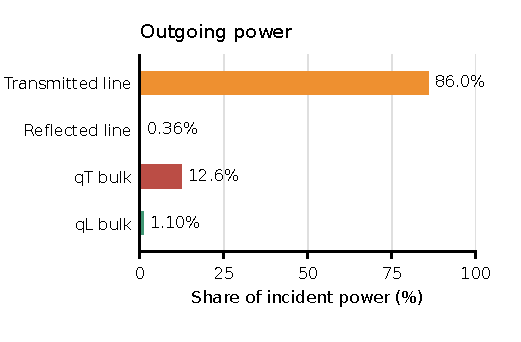
\includegraphics[width=0.55\textwidth]{figures/figure4_reference_power.pdf}
 \caption{Percentage of incident line power in each outgoing channel for the six-segment reference taper at the reference frequency $\omega\sqrt{m_b/K_{\rm diag}}=1.2$. The two bulk bars separate shear-like and longitudinal-like radiation. The reference calculation uses $N=192$ reciprocal-grid points per axis and order $M=256$ for the principal-value (PV) reconstruction. The companion panel comparing the three methods appears in Supplementary Material Sec.~SM4.}
 \label{fig:s6-reference}
\end{figure*}

For the same taper and line stiffness, the left panel of Fig.~\ref{fig:s9-frequency-partition} shows all four outgoing fractions from $\omega=0.6$ to $1.8$. The right panel compares qT conversion with the fixed-contact law in Eq.~\eqref{pred:eq-lowfreq}. The ratio to $C_T\omega^2$ is $1.04$ at $\omega=0.2$ and $1.17$ at $0.4$, but falls to $0.316$ at the benchmark $\omega=1.2$. At all 49 sampled frequencies from $0.6$ to $1.8$, more than $10\%$ of incident power reaches qT modes. The smallest sampled value is $10.5\%$ at $\omega=1.575$, and the largest is $21.8\%$ at $\omega=0.825$. The samples establish conversion at multiple frequencies and leave the behavior between them unresolved. Supplementary Material Sec.~SM5A also varies the line stiffness (and hence wave speed), bulk stiffness ratio, contact length and spring profile in separate finite scans. These comparisons keep the line and bulk masses fixed.

\begin{figure}[!htbp]
 \centering
 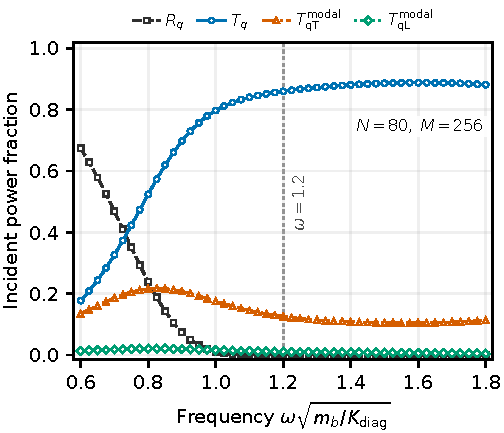
\includegraphics[width=0.485\linewidth]{figures/paper1_frequency_partition.pdf}\hfill
 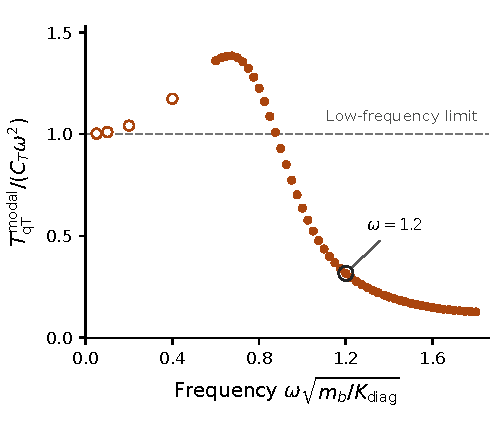
\includegraphics[width=0.485\linewidth]{figures/paper1_low_frequency_ratio.pdf}
 \caption{Frequency dependence for the fixed six-segment reference taper. The left panel shows fractions of incident line power for the 49 surface calculations ($N=80$, PV order $M=256$). Connecting lines guide the eye. The right panel shows qT conversion divided by its leading low-frequency value. Open circles show the low-frequency calculations of Supplementary Material Sec.~SM7A and filled circles show the same scan as on the left. The dashed line is the limiting ratio of one. The vertical line (left) and ring (right) mark $\omega=1.2$, where the stiffness bounds of Sec.~\ref{sec:s9-robustness} apply. Both panels sample the propagating line band $0<\omega<2.6$.}
 \label{fig:s9-frequency-partition}
\end{figure}

\paragraph*{Redistributing a fixed total spring stiffness.}
Compare the reference profile with
$\bm g_{\rm end}/K_{\rm diag}=(0.5,0,0,0,0,0.5)$ at $\omega=1.2$.
The bare line and bulk, six available segment positions, and connected
seven-site line region are unchanged.  Both profiles have
$\sum_sg_s=K_{\rm diag}$ and total physical source-spring stiffness
$8K_{\rm diag}$.  Their active spring counts are 48 and 16, and their
largest individual spring stiffnesses are $0.2K_{\rm diag}$ and
$0.5K_{\rm diag}$, respectively; the comparison therefore fixes total
stiffness and extent, not every fabrication resource.  Each profile is
solved with its complete reciprocal contact loading.

\begin{table}[t]
 \squeezetable
 \caption{Reference taper and endpoint-only contact at equal total spring stiffness $8K_{\rm diag}$ and $\omega=1.2$, evaluated
 with the same $N=192$ surface/$M=256$ PV matrices.  The two modal powers
 are fractions of incident line power; the final column is the qT share
 of emitted bulk power.  Shares are calculated before rounding.  These
 are numerical estimates, not certified bounds.}
 \label{tab:s6-equal-total}
 \begin{ruledtabular}
 \begin{tabular}{lccc}
 Profile & $T_{\qT}^{\rm modal}$ & $T_{\qL}^{\rm modal}$
 & $T_{\qT}^{\rm modal}/T_{\rm bulk}$\\
 \hline
 Reference & 0.1257 & 0.01102 & 0.9194\\
 Endpoint-only & 0.1586 & 0.02449 & 0.8662\\
 \end{tabular}
 \end{ruledtabular}
\end{table}

The five-profile scan in Supplementary Material Sec.~SM5A found higher conversion for a uniform profile ($g_j=0.20K_{\rm diag}$) than for the reference taper, while varying both the total stiffness and its distribution. With the total held fixed in Table~\ref{tab:s6-equal-total}, concentrating the springs at the two ends raises incident-to-qT conversion by about 3.3 percentage points. The qT share of bulk emission falls by about 5.3 percentage points because qL power increases by a larger factor than qT power. This comparison concerns two fully loaded contacts at one frequency. The two profiles have the same leading low-frequency coefficients in Eq.~\eqref{pred:eq-lowfreq}. Supplementary Material Sec.~SM4 gives all four outgoing fractions and the numerical inputs for both profiles. The tolerance guarantee for the reference taper (Sec.~\ref{sec:s9-robustness}) applies to that contact alone. An exact-lattice error enclosure for the endpoint-only result remains open.

\paragraph*{Changing the strength and distribution of the contact springs.}
Table~\ref{tab:s6-coupling-comparison} compares five fully loaded reciprocal contacts at $\omega=1.2$ and $K_q/K_{\rm diag}=1.69$, with the same bare bulk and 48 active springs on six motifs. The doubled and scaled tapers multiply every reference link stiffness by two and three, respectively. The uniform profile has $g_j/K_{\rm diag}=0.5$ on all six motifs. The increasing ramp has $g_j/K_{\rm diag}=j/7$ for $j=1,\ldots,6$, starting from the incident lead. The total stiffness of the physical springs is $8\sum_jg_j$.

\begin{table}[!htbp]
 \centering
 \caption{Contact comparison at $\omega=1.2$ using the same bare-bulk $N=192$ surface/$M=256$ principal-value matrices. Total spring stiffness and peak individual link stiffness are in units of $K_{\rm diag}$. Both power columns give rounded numerical estimates as percentages of incident line power. The text gives separate qT bounds for the reference taper and ramp. The increasing ramp is driven from its softer end.}
 \label{tab:s6-coupling-comparison}
 \begin{ruledtabular}
 \begin{tabular}{lcccc}
 Profile & Total stiffness & Peak link stiffness & Reflected & qT conversion\\
 \hline
 Reference taper & $8$ & $0.2$ & $0.36\%$ & $12.6\%$\\
 Doubled taper & $16$ & $0.4$ & $4.4\%$ & $52.2\%$\\
 Scaled taper & $24$ & $0.6$ & $24.3\%$ & $62.7\%$\\
 Uniform & $24$ & $0.5$ & $16.7\%$ & $67.8\%$\\
 Increasing ramp & $24$ & $6/7$ & $12.0\%$ & $73.6\%$\\
 \end{tabular}
 \end{ruledtabular}
\end{table}

The reference taper and the ramp differ in both total and peak stiffness. At equal total stiffness, the last three rows of Table~\ref{tab:s6-coupling-comparison} show how redistribution changes conversion while peak link stiffness still varies. From the scaled taper to the ramp, reflection falls by $12.3$ percentage points and qT conversion rises by $10.9$ points. The balance goes to the continuing line and qL modes. Driving the same ramp from its stiffer end raises reflection to about $39\%$ and lowers qT conversion to $48.4\%$. For incidence from either end, $7.6\%$ reaches the opposite lead, as reciprocity requires [Eq.~\eqref{eq:reciprocity}]. Supplementary Material Sec.~SM5D gives the complete soft-end partition at $\omega=1.2$ and the unperturbed ramp's qT conversion at the fourteen frequencies used for the packet comparison. The largest of these fourteen estimates is about $77.6\%$ at $\omega\simeq1.3585$. The ramp came from a finite profile-and-strength scan. These results establish neither a global optimum nor performance throughout a band.

The evidence scopes differ. At $\omega=1.2$, the reference taper satisfies $T_{\qT}^{\rm modal}>0.1037$ when its six motif strengths vary independently by up to $5\%$ about their unperturbed values. All eight springs in each motif share one factor (SM5B). For the doubled taper, scaled taper and uniform profile, Table~\ref{tab:s6-coupling-comparison} reports numerical power estimates. For the ramp at its stated strengths, the separate exact-lattice enclosure is $0.732166<T_{\qT}^{\rm modal}<0.739652$ (SM5D). It contains the numerical estimate but does not certify its rounding to $73.6\%$. A second ramp certificate guarantees $T_{\qT}^{\rm modal}>0.69$ under the same relative variations about the ramp's own six unperturbed motif strengths. These tolerance guarantees apply at $\omega=1.2$; they do not cover 48 independent spring errors or a frequency band.

The fraction of incident line power radiated into the bulk rises from $13.7\%$ for the reference taper to $80.4\%$ for the ramp. The qT share of that emission changes only from $91.9\%$ to $91.5\%$. Thus, at this frequency the ramp sends more line power into the bulk while the radiated mixture remains predominantly qT. The angular and source-sector comparisons below return to the reference contact unless stated otherwise.

\subsection{Angular collection of the generated power}
\label{pred:sec-collection}

For the reference junction, projecting the polarization perpendicular to each wavevector gives the geometric diagnostic $T_{\perp k}^{\rm geom}\simeq0.12563$, close to the modal qT fraction. To determine where the energy travels, we sort the bulk power by group velocity. All eight octants receive power, with about $1.3\%$ of total bulk emission in the least populated one. The qT modes themselves also carry energy into every octant. At both grid resolutions ($N=80$ and $96$) the least populated octant receives about $1.4\%$ of all emitted qT power. Of the total power emitted into all three bulk branches, about $94\%$ travels more than $30^\circ$ from both the forward and backward line directions. With the same total-bulk weighting, the median of $\sin\theta$ is about $0.86$, where $\theta$ is the angle from the forward axis. On both grids, summing over directions recovers the total emitted power for the same scattering state within $0.022\%$.

How much of the radiation travels forward? An ideal far-field collector accepts waves whose energy flows within a cone of half-angle $\Theta$ about the incident direction $+x$. In the spectral integral of Eq.~\eqref{eq:s5-cluster-spectral}, this selects the shell modes with $v_{g,\lambda,x}/|\bm v_{g,\lambda}|\geq\cos\Theta$. Dividing the qT and qL powers in that cone by incident line power gives $T_{\qT,\Theta}$ and $T_{\qL,\Theta}$. The fraction of collected power carried by qT is
\begin{equation}
 \eta_{\qT,\Theta}
 =\frac{T_{\qT,\Theta}}{T_{\qT,\Theta}+T_{\qL,\Theta}}.
 \label{pred:eq-cone-share}
\end{equation}
To find how much of all emitted qT power reaches the cone, divide its qT power by the qT power radiated in every direction. This gives $T_{\qT,\Theta}/T_{\qT}^{\rm modal}$. At the reference frequency, the centered source has zero overlap with qT modes whose wavevector is parallel to the line. The cone selects the direction of energy flow, which can differ from the wavevector in this anisotropic lattice. Waves with oblique wavevectors can therefore contribute to collection near the axis.

\begin{table}[tb]
 \centering
 \caption{Numerically evaluated forward-cone collection at $\omega=1.2$, for the complete six-motif reference junction, profile in Eq.~\eqref{eq:s2-g-profile}, and $s=1$. The two powers are fractions of incident line power; the final column is their qT share. Angles select group velocity, not wavevector. These are ideal asymptotic modal powers, not measurements of a loaded receiver.}
 \label{pred:tab-cone}
 \begin{tabular}{cccc}
 \toprule
 $\Theta$ & $T_{\qT,\Theta}$ & $T_{\qL,\Theta}$ & $\eta_{\qT,\Theta}$\\
 \midrule
 $10^\circ$ & $9.17\times10^{-6}$ & $7.61\times10^{-4}$ & $1.19\%$\\
 $20^\circ$ & $1.99\times10^{-4}$ & $2.69\times10^{-3}$ & $6.89\%$\\
 $30^\circ$ & $2.87\times10^{-3}$ & $5.09\times10^{-3}$ & $36.1\%$\\
 \bottomrule
 \end{tabular}
\end{table}

At $\omega=1.2$, qT carries $91.9\%$ of all bulk emission and $1.19\%$ of the power in the $10^\circ$ forward cone (Table~\ref{pred:tab-cone}). This cone intercepts only about $0.0073\%$ of all emitted qT power. Keeping only the strain-driven radial coupling and solving that modified junction raises the qT share in the cone to $99.2\%$. The qT power reaching it falls to $8.84\times10^{-7}$ of incident power, about one tenth of the complete junction's $9.17\times10^{-6}$.

Direct cone quadrature and a separate angular calculation agree on the sampled contributions. Both use the same source force calculated from the coupled response. Angular refinement does not bound the uncertainty in the principal-value input to this force, and the numerical search may miss very narrow sets of wavevectors that send energy into the cone (Supplementary Material Sec.~SM7B).

The low-frequency law in Eq.~\eqref{pred:eq-lowfreq} predicts the cone powers analytically under its fixed-contact assumptions. Take $\omega\to0$ at a fixed opening angle $0<\Theta\leq\pi/2$ and put $c=\cos\Theta$. Then
\begin{align}
 T_{\qT,\Theta}&=C_T\omega^2\frac{2-3c+c^3}{4}+o(\omega^2),\nonumber\\
 T_{\qL,\Theta}&=C_L\omega^2\frac{1-c^3}{2}+o(\omega^2).
 \label{pred:eq-cone-lowfreq}
\end{align}
Here $\theta$ is the angle between propagation and the line. The factors multiplying $C_T$ and $C_L$ are the cone integrals of $\sin^2\theta$ and $\cos^2\theta$, respectively, divided by the corresponding full-sphere integrals. The group directions and polarization projectors approach their isotropic acoustic limits, so these factors apply to energy collected by direction. The limiting qT shares at $10^\circ$, $20^\circ$ and $30^\circ$ are $7.39\%$, $24.6\%$ and $43.3\%$, respectively. The table gives the corresponding finite-frequency results. Taking $\Theta\to0$ in radians only after the frequency limit gives a narrow-cone share asymptotic to $\tfrac12(c_L/c_T)^3\Theta^2$. A simultaneous limit, or a narrowing aperture at fixed frequency, would require separate analysis. A finite-distance detector would also require its coherent overlap, local interference and loading to be accounted for.

\subsection{Mechanism controls and elastic interpretation}
\label{sec:s6-controls}

An axial force can launch shear-like motion obliquely to the line, and the strain-driven radial forces can radiate through the same springs. To determine what each contributes, we first change which coupling acts and solve for the resulting motion. Section~\ref{sec:s3-mechanism} identified the axial coupling $X$ to mean endpoint displacement and the radial coupling $R$ to segment strain. Table~\ref{tab:s6-ablation} compares the physical contact $H_c=H_X+H_R$ with two controls that keep only $H_X$ or only $H_R$. The bare line and bulk $H_q+H_b$ are common to all three. The independent $N=192$ tetrahedron calculation solves each Hamiltonian with its own line self-stiffness, corner stiffness and reciprocal coupling. Because the scattering states change, the two control powers need not add to the full power.

\begin{table}[t]
 \squeezetable
 \caption{Source-channel controls for the reference taper at $\omega=1.2$, with frequency conjugate to $\tau$. The full row uses the physical paired-link Hamiltonian and the $X$-only and $R$-only controls use positive surrogate Hamiltonians. The three rows give rounded estimates from the $N=192$ tetrahedron calculation. Its full-contact incident-to-qT fraction is $0.1256$, compared with $0.1257$ by surface integration in Table~\ref{tab:s6-equal-total}. Shares are calculated before rounding.}
 \label{tab:s6-ablation}
 \begin{ruledtabular}
 \begin{tabular}{lccc}
 Hamiltonian & $T_{\rm bulk}$ & $T_{\qT}^{\rm modal}$ & $T_{\qT}^{\rm modal}/T_{\rm bulk}$\\
 \hline
 Full $X+R$ & 0.1366 & 0.1256 & 0.9194\\
 $X$ only & 0.1152 & 0.1022 & 0.8873\\
 $R$ only & 0.002430 & 0.002231 & 0.9179\\
 \end{tabular}
 \end{ruledtabular}
\end{table}

With $R$ alone, the surface calculation gives positive qT output at all five tested frequencies, $\omega=0.8$, $1.0$, $1.2$, $1.4$ and $1.7$. Radial coupling can thus radiate qT on its own, although its isolated output is small at the reference point. To test its effect in the presence of $X$, vary the contact energy according to
\begin{equation}
\begin{aligned}
 H_c(\alpha)&=H_X+\alpha H_R,\\
 H(\alpha)&=H_q+H_b+H_c(\alpha),
 \qquad0\leq\alpha\leq1.
\end{aligned}
 \label{eq:s6-alpha-family}
\end{equation}
Here $\alpha$ scales the entire radial spring energy, including all its force and stiffness terms. The paired-spring contact has $\alpha=1$. Smaller values define diagnostic controls. At the reference frequency, we solved the scattering problem at 21 sampled values of $\alpha$. The resulting $T_{\qT}^{\rm modal}$ increases from about $0.1022$ to $0.1256$ across those samples. The scan leaves the behavior between samples open (SM4).

We can also keep the full physical scattering state fixed and ask how the two force components interfere. Split its source block as $V=V_X+V_R$ and apply the same corner response and the same line displacement to each part,
\begin{equation}
\begin{aligned}
  \veta_\nu&=(I+Ug_0^R)^{-1}V_\nu\vchi_D^{(L)},
  &&\nu\in\{X,R\},\\
  \veta&=\veta_X+\veta_R.
\end{aligned}
  \label{eq:s6-same-state-source}
\end{equation}
With $Q_{\qT}=\ImH g_{0,\qT}^R$, define
\begin{equation}
\begin{aligned}
  T_{\nu\nu}&=2\veta_\nu^\dagger Q_{\qT}\veta_\nu,
  &&\nu\in\{X,R\},\\
  T_{XR}&=4\operatorname{Re}
  \left(\veta_X^\dagger Q_{\qT}\veta_R\right).
\end{aligned}
  \label{eq:s6-same-state-terms}
\end{equation}
The invariant modal-qT quadratic form then obeys the exact algebraic identity
\begin{equation}
 T_{\qT}^{\rm modal}=T_{XX}+T_{RR}+T_{XR}.
 \label{eq:s6-same-state-XR}
\end{equation}
The reference surface/PV calculation gives
\begin{equation}
 \begin{split}
 (T_{XX},T_{RR},T_{XR})\simeq{}&
 (0.10148,0.0017918,\\
 &0.022389).
 \end{split}
\end{equation}

The self terms measure the qT radiation from each force component evaluated with the motion of the full junction. The cross term measures interference between the components. Here it is constructive and accounts for about $17.8\%$ of the full qT power. Only the sum gives the qT output of the coupled junction. Supplementary Material Sec.~SM4 gives the independent tetrahedron check.

Adding $H_R$ in the tetrahedron calculation raises conversion by about $2.34$ percentage points of incident power (Table~\ref{tab:s6-ablation}). This change includes the response of the axial force to the new motion of the line and corners. The interference calculation evaluates both forces with that motion already fixed.

The same radial coupling can also lower conversion. Keep the six-motif profile and bulk fixed, and choose $\omega=0.8$ and $c_q=0.8$ ($K_q/K_{\rm diag}=0.64$). The surface solution then gives $T_{\qT}^{X\text{-only}}\simeq0.3625$ and $T_{\qT}^{\rm full}\simeq0.3507$. The full-state interference term is positive, $T_{XR}\simeq+0.01828$, yet adding $H_R$ reduces qT output by about $1.18$ percentage points of incident power. The axial self term falls by more than the radial self term and the interference term contribute together. An independent tetrahedron calculation reproduces the sign and magnitude (Supplementary Material Sec.~SM7C).

For one complete motif a symmetry argument gives an exact result. Take identical endpoint masses and bare diagonal stiffnesses, identical scalar leads and an axially reflection-symmetric bulk. Endpoint-symmetric motion couples to $X$, and endpoint-antisymmetric motion to $R$. These two blocks evolve independently, so removing one entire sector, including its reciprocal self-stiffness, leaves the other block intact. For a bulk cluster $C$ integrated over a whole shell invariant under axial reflection,
\begin{equation}
 T_C^{\rm full}=T_C^{X\text{-only}}+T_C^{R\text{-only}},
 \qquad T_{XR,C}=0.
 \label{eq:s6-one-motif-additivity}
\end{equation}
All three powers have the same one-sided incident-power denominator. Within this symmetric family, a reduction in whole-shell qT output on adding $R$ therefore requires at least two motifs. Two motifs alone do not ensure a reduction. Reflected and transmitted line amplitudes can still interfere, and a one-sided collector can break the reflection symmetry of the observed bulk sector. Supplementary Material Sec.~SM7C gives the block proof and the bound of one half of incident power for each isolated sector.

An isotropic elastic calculation provides a comparison for the large qT share. A time-harmonic axial point force in an unbounded isotropic elastic medium radiates shear power $P_S$ and compressional power $P_P$ in the ratio~\cite{Achenbach1973,Graff1975,Schmidt2018ElasticPurcell}
\begin{equation}
 \frac{P_S}{P_P}=2\left(\frac{c_L}{c_T}\right)^3.
 \label{eq:s6-point-force}
\end{equation}
With $c_L/c_T=\sqrt3$, shear carries about $91.2\%$ of the point force's radiated power. To include the spatial extent of the source, prescribe the six-segment line wave and apply its axial and radial forces to the isotropic continuum (first Born approximation). Shear carries about $87.5\%$ of the emitted power for the axial forces alone and $91.8\%$ for the radial forces alone. Adding their radiated powers without interference gives $87.6\%$. Combining the forces with their relative phase gives $91.9\%$, because shear interference is constructive and compressional interference is destructive. Finite axial and radial line sources give a related comparison~\cite{Aldridge1998}.

The prescribed six-segment continuum source and the coupled lattice in Fig.~\ref{fig:s6-reference} thus both put about $92\%$ of emitted power into shear or shear-like modes. Ordinary elastic radiation can account for a large shear share. Conversion of incident line power additionally depends on how strongly the junction radiates into the bulk. The continuum calculation prescribes the source, while the lattice calculation determines it from the motion of both line and bulk. The two calculations also use different polarization projectors. Taking the weak-coupling limit of the discrete lattice at this fixed frequency gives a qT share of $92.7\%$ for the selected numerical kernel [Eq.~\eqref{eq:weak-share}]. The externally actuated shear sources discussed in Sec.~\ref{sec:scope} likewise report different output measures~\cite{Liang2026MetaExcitation,Lu2026ThreeDimensional}. Comparing incident-line efficiencies would require a common incident power and output channel.

Supplementary Material Sec.~SM4 gives the angular-power prescription, continuum cross terms and comparison with the lattice. The validation archive supplies the machine-readable values and code.

\subsection{Frequency-controlled upstream bulk radiation}
\label{sec:pred-backward}

To isolate the effect of frequency on direction, hold a contact of 24 consecutive motifs fixed on a stiffer line. Each link has stiffness $0.1K_{\rm diag}$ in the two end motifs and $0.2K_{\rm diag}$ in the 22 interior motifs. The line has $c_q=1.5$ ($K_q/K_{\rm diag}=2.25$), placing its upper band edge at $\omega=3$ in reference units. For incidence along $+x$, upstream bulk power sums the outgoing modes with negative axial group velocity. Reflection along the line is counted separately in $R_q$. The fractions of incident line power radiated upstream are
\begin{equation}
 T_-(2.6)\simeq0.17,\qquad T_-(2.9)\simeq0.710.
 \label{eq:s6-upstream-control}
\end{equation}
As shares of emitted bulk power, the upstream values are $51.5\%$ and $98.5\%$, respectively. At $\omega=2.6$ the bulk branches meet on the frequency shell, and the directional sum includes all branches. At $2.9$, above the lower pair's upper edge $2\sqrt{2}$, only the upper branch radiates, and its displacement need not be parallel to its wavevector. The 24-motif example selects bulk power by direction. The six-motif ramp's estimated $73.6\%$ at $\omega=1.2$ measures qT power summed over all directions and divided by incident line power (Table~\ref{tab:s6-coupling-comparison}). Backward elastic conversion has precedents in structured media~\cite{Chaplain2020}. SM7E gives the contact parameters, branch-edge proof and stationary cross-checks. A rigorous combined error enclosure and a packet test at $2.9$ remain open.

\section{Real-time packet corroboration}
\label{sec:s7-direct}

When a longitudinal pulse reaches the contact, how much of its energy appears in the two shear-like (qT) bulk modes? We launch the same pulse at the six-segment reference taper and at the stronger increasing ramp of Table~\ref{tab:s6-coupling-comparison}. During the selected time intervals, the three-dimensional bulk stores about $14\%$ of the initial line energy for the taper and $78\%$ for the ramp. In each case the qT modes account for $91$--$92\%$ of the mean bulk modal energy. The ramp therefore puts much more energy into the bulk, with a similar division between polarizations. Both the total spring stiffness and its distribution along the contact change between these two examples.

\begin{table}[!ht]
 \centering
 \caption{qT response of the two contacts. The carrier column gives the fraction of incident line power at $\omega_0=1.2$. The packet prediction weights surface qT conversions at fourteen distinct frequencies by the initial energies of the corresponding Fourier modes. The in-band sum is divided by the full initial periodic line energy, then rescaled to the initial open-line normalization without changing the displayed percentages. The direct result is the mean stored qT energy over each contact's reporting interval, divided by the initial open-line energy.}
 \label{tab:s7-packet-comparison}
 \begin{ruledtabular}
 \begin{tabular}{lccc}
 Contact & Carrier power & \shortstack{Packet prediction\\(evaluated band)} & \shortstack{Direct packet\\(mean stored energy)}\\
 \hline
 Reference taper & $12.6\%$ & $12.77\%$ & $12.76\%$\\
 Increasing ramp & $73.6\%$ & $71.63\%$ & $71.65\%$\\
 \end{tabular}
 \end{ruledtabular}
\end{table}

Frequency averaging raises the taper result slightly and lowers the ramp result relative to the carrier. A related packet study resolved polarization conversion at a nanotube--graphene junction~\cite{Shi2018}.

\subsection{Launching the packet and measuring the bulk response}
\label{sec:s7-packet}

At launch, the line carries the packet energy, with a negligible additional amount stored in the contact springs. A Gaussian envelope of width $7a$ modulates a longitudinal carrier at $\omega_0=1.2$. The packet starts to the left of the contact. We choose its initial velocities from the line dispersion so that the propagating part travels to the right. At time $\tau=0$, the bulk is at rest at its equilibrium positions. We advance the line and the three-dimensional bulk together with a symmetric Verlet integrator~\cite{Verlet1967}. Both lattices have free boundaries and evolve without external forcing or damping. The initial energy of the open line, $E_0=H_q(0)$, sets the scale for the reported bulk energies.

Summing the bond current [Eq.~\eqref{eq:bondcurrent}] once per contact spring from line to bulk gives $J_{q\to b}$. Assigning half the contact energy $E_{\rm link}=H_c$ [Eq.~\eqref{eq:s2-Hc-total}] to each side gives
\begin{equation}
 \int_0^\tau J_{q\to b}(\tau')\,d\tau'
 =\Delta E_b(\tau)+\frac12\Delta E_{\rm link}(\tau).
 \label{eq:s7-current-balance}
\end{equation}
Here $E_b$ is the open-bulk energy and $\Delta E$ denotes the change since launch. This balance checks total transfer. To resolve polarization, we treat each whole-bulk snapshot as periodic and Fourier transform its displacements and velocities~\cite{BornHuang1954}. Summing the energies of the two lower branches gives $E_{\qT}^{\rm per}(\tau)$. At exact degeneracies with the upper branch we use the midpoint of the allowed lower-pair allocations (SM5C).

We average $E_{\qT}^{\rm per}/E_0$ over the longest interval that passes five checks on the direct evolution, including small residual contact energy and current. The stationary predictions enter only after the interval is selected. For the taper it spans $52.8\le\tau\le55.4$ (Fig.~\ref{fig:s7-dynamics}). Supplementary Material Sec.~SM5C gives the five thresholds, sampling and averaging rules, and the separate check of all six faces.

\begin{figure}[t]
 \centering
 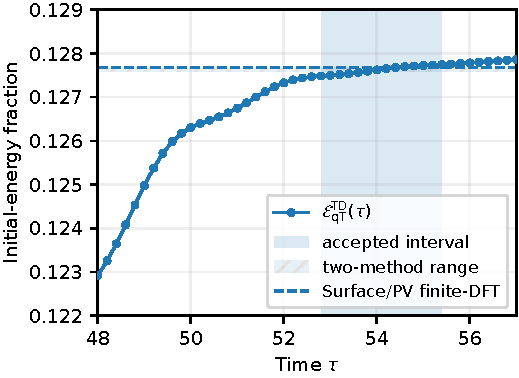
\includegraphics[width=0.55\linewidth]{figures/paper1_sectionVII_fig6a_qT_window_v2.pdf}
 \caption{Fraction of initial open-line energy stored in the reference taper's bulk qT modes, $\mathcal E_{\qT}^{\rm TD}(\tau)=E_{\qT}^{\rm per}(\tau)/E_0$, at time $\tau$ in units of $\sqrt{m_b/K_{\rm diag}}$. Averaging the dots over the shaded interval gives the direct result in Table~\ref{tab:s7-packet-comparison}. The dashed line gives the surface prediction. The hatched band spans the in-band surface and tetrahedron estimates.}
 \label{fig:s7-dynamics}
\end{figure}

\subsection{Comparison with the stationary prediction}
\label{sec:s7-result}

In this linear, time-independent junction each frequency scatters independently. Weight its stationary incident-power fraction $T_C(\omega)$ for bulk sector $C$ by the initial line energy $W(k)$ in each bin of the signed Fourier grid $\mathcal G$. With $\mathcal P$ the propagating bins ($0<|k|a<\pi$), the predicted packet fraction for sector $C$, here the qT pair, is
\begin{equation}
 T_C^{\rm packet}
 =\frac{\displaystyle\sum_{k\in\mathcal P}W(k)T_C[\omega_q(k)]}
 {\displaystyle\sum_{k\in\mathcal G}W(k)}.
 \label{eq:s7-packet-average}
\end{equation}
The conjugate bins $k$ and $-k$ represent one real right-moving wave and use the same left-incident coefficient. For Table~\ref{tab:s7-packet-comparison}, fourteen frequencies in $0.8\le\omega\le1.6$ account for $99.968\%$ of the initial periodic line energy. By passivity, the energy fraction outside this band bounds the omitted contribution. The zero-frequency bin carries no energy. The Nyquist bin has zero group velocity and contributes only to the denominator. Converting to $E_0$ leaves the displayed percentages unchanged (SM5C and SM5D).

Using the unrounded results, the direct value minus the stationary in-band prediction is about $-0.005$ percentage points for the taper and $+0.015$ percentage points for the ramp. The taper's direct estimate falls between the surface and tetrahedron predictions, slightly below the surface result even before any omitted spectral contribution is added (SM5C).

The initial ramp run yielded no qualifying interval of sufficient duration. Widening the bulk transversely and extending the time search, with the same thresholds and minimum duration, gave $57.4\le\tau\le64.2$. On this fixed interval, a further increase in the transverse dimensions lowered the direct estimate from $71.65\%$ to $71.63\%$, just below the unrounded stationary prediction. SM5D gives the bulk dimensions, timestep and sampling controls. Their differences give no combined error bound. The $73.6\%$ estimate and its bounds apply to monochromatic input at the carrier.

The packet comparison tests the stationary calculation by following the same harmonic lattice through time. Its direct observable is the energy stored throughout the bulk during the selected interval. A polarization-resolved flux at a particular location or a signal at a distant detector requires a separate measurement.

\section{Robustness, scaling, and model scope}
\label{sec:s9-robustness}

At $\omega=1.2$, the fraction of incident line power entering qT remains above $10.37\%$ for the reference taper and above $69\%$ for the increasing ramp of Table~\ref{tab:s6-coupling-comparison} when each contact's six motif strengths vary independently by up to $5\%$.

The bounds allow $g_j=g_j^\star(1+\delta_j)$, with $|\delta_j|\leq0.05$ independently for $j=1,\ldots,6$. The eight springs of motif $j$ share its factor. The ramp has $g_j^\star=(j/7)K_{\rm diag}$ in order from the incident lead. The geometry and bare media stay fixed, so the same enclosures of the infinite bulk's Green and qT spectral matrices apply to both contacts. For each contact an inverse-perturbation estimate bounds the change in qT output throughout the six-dimensional box, including the force that the bulk exerts back on the line (Supplementary Material Secs.~SM5B and SM5D). Independent changes to all 48 springs and a continuous range of frequencies would require further bounds.

We also sampled the reference taper's stiffness box at eleven frequencies from $1.10$ to $1.30$. At each frequency all 193 settings---the unperturbed reference taper, its 64 box corners and 128 interior settings---exceeded the illustrative target of $10\%$ incident-to-qT conversion. A second integration method repeated the test at three frequencies. Both methods found the smallest sampled conversion at $\omega=1.30$ with all six strengths at their lower limits (SM7D). At $\omega=1.2$ the proof covers every combination in the box. At the other ten sampled frequencies the result applies to the settings evaluated. Whether the target holds throughout the band remains open.

The parameter survey of Supplementary Material Sec.~SM5A varied frequency, overall coupling, contact length, stiffness profile, line speed and the ratio of diagonal to axial bulk stiffness, one family at a time. Its 85 positive-coupling calculations included repeated reference settings. All gave positive qT output.

The reference taper was chosen as a simple symmetric contact with end springs half as stiff as the interior springs. Whether that choice preceded inspection of exploratory qT results remains undocumented. At $\omega=1.2$, the five profiles in SM5A converted about $6.5\%$ to $15.8\%$ of incident line power into qT modes. The taper gave $12.6\%$, and the uniform profile gave the largest sampled value. Total spring stiffness differed across the five profiles.

At fixed $\omega=1.2$, multiplying every taper stiffness by $s=1,1.5,2$ gave about $12.6\%$, $30.9\%$ and $52.2\%$ qT conversion. At the weakest tested scale, $s=0.05$, the fraction was only $0.025\%$. At twice the reference stiffness, about $38.4\%$ of the incident power continued on the line, $4.4\%$ was reflected and $5.0\%$ entered the upper bulk branch. About $57.2\%$ entered the bulk altogether. For $s=1,1.5,2$, stronger coupling reduced forward line transmission while the qT share of radiated bulk power stayed above $91\%$. SM5A gives the six sampled families, solver settings and energy-balance checks. The fixed-total-stiffness comparison in Table~\ref{tab:s6-equal-total} and the increasing ramp are separate from those 85 calculations.

The line-speed scan of Sec.~\ref{sec:s2-units-nullspaces} varied $K_q$ at fixed masses. To test the sensitivity to line mass, we held $K_q/K_{\rm diag}=1.69$, the reference taper, the bulk and $\omega=1.2$ fixed. Changing the mass of every line site, including both leads, to give $m_q/m_b=0.75,1,1.25$ yielded about $19\%$, $12.6\%$ and $9.1\%$ incident-to-qT conversion, respectively. The $10\%$ target is therefore missed in the heavier-line example. Both the incident wavelength and the line's response to the junction change with mass. The spring-tolerance guarantee holds the masses fixed. The validation archive gives the four power fractions and the independent tetrahedron comparison.

For the reference taper at $\omega=1.2$, the leading force from the uncoupled line overlaps a qT mode on a regular patch of the frequency shell (SM3). Thus $\mathcal A_{\qT}>0$ in Eq.~\eqref{eq:weak}, and qT conversion is positive for sufficiently small $s>0$ and vanishes quadratically as $s\to0^+$. Section~\ref{pred:sec-lowfreq} instead lowers frequency at fixed strength. Near the finite reference contact, the lead, bulk and coupled response and the separated qT spectral measure are continuous away from lead thresholds, bulk shell stationary points, lower--upper branch-gap closures and coupled-response poles. The verified regularity margins therefore preserve positive qT output for sufficiently small parameter changes at fixed connectivity, contact positions and bond inventory. The size of this neighborhood is unquantified. The six-factor box above has explicit bounds, and the length survey separately samples changes to the graph.

\subsection{Scaling and effective-model status}
\label{sec:s9-scaling-scope}

Choosing $a=0.25,0.5,1,2$ or $4$ expresses one nondimensional reference calculation in five sets of dimensional units. A separate similarity law compares time-independent systems on the same graph with the same bond geometry. Let $\mathsf M$ and $\mathsf K$ be the mass and stiffness matrices of the entire system, including the leads and the contact springs. Scale them by positive factors, $\mathsf M'=\alpha_M\mathsf M$ and $\mathsf K'=\alpha_K\mathsf K$, and set $\Omega_{\rm sc}=\sqrt{\alpha_K/\alpha_M}$. With both frequencies expressed in the original system's units, the corresponding channels satisfy
\begin{equation}
 T'_C(\Omega_{\rm sc}\omega)=T_C(\omega),
 \qquad C\in\{q,\qT,\qL\}.
 \label{eq:s9-complete-scaling}
\end{equation}
Reflection also has the same power fraction. The rescaled displacement $\vx'(\tau)=\vx(\Omega_{\rm sc}\tau)$ multiplies every bond force by $\alpha_K$ and every velocity by $\Omega_{\rm sc}$ at the corresponding phase and equal incident displacement amplitude. All powers thus acquire the same factor $\alpha_K\Omega_{\rm sc}$, which cancels in their ratios.

Now scale all masses and the bare line and bulk stiffnesses, keeping the junction springs fixed. Write $\mathsf K=\mathsf K_{\rm bare}+\mathsf K_c$, where the two matrices are the displacement Hessians of $H_q+H_b$ and $H_c$. Factoring $\alpha_K$ out of $\mathsf K'=\alpha_K[\mathsf K_{\rm bare}+\alpha_K^{-1}\mathsf K_c]$ gives
\begin{equation}
 T'_C(\Omega_{\rm sc}\omega)
 =T_C(\omega;s=\alpha_K^{-1}).
 \label{eq:s9-partial-scaling}
\end{equation}
Changing the bare propagation rates with fixed junction springs therefore reproduces the original coupling scan at $s=1/\alpha_K$ and corresponding frequencies.

Which force components can the prescribed line motion supply at long wavelengths? For a non-axial bulk wavevector, SV and SH are transverse directions in and perpendicular to the plane containing the line axis and that wavevector. In the bare-source calculation of SM1, hold the line's Bloch displacement amplitude $Q$, spacing $a$, stiffness profile and number of segments fixed, and write $(a\vk,a\kappa)=\varepsilon(\bm d,b)$. Here $\vk$ is the bulk wavevector, $\kappa$ the line wave number, and the non-axial vector $\bm d$ and scalar $b$ are fixed and dimensionless. As $\varepsilon\to0^+$ along a regular direction, the complex projections of the axial-average ($X$) and radial segment-strain ($R$) forces obey
\begin{align}
V_X^{SV}&=\order(1),\\
V_R^{SV}&=\order(\varepsilon^2),
&V_R^{SH}&=\order(\varepsilon^4).
\label{eq:s9-source-orders}
\end{align}
The leading radial force lies in the axis--wavevector plane, so a radial SH projection can first appear at fourth order. Its coefficient can vanish in symmetry directions. These geometric projections describe the source before the bulk reacts. A finite-frequency power fraction also requires the coupled line motion and the actual bulk eigenmodes. Section~\ref{sec:s4-bulk-symmetry} gives a separate polarization bound for the homogeneous bulk with equal axial and diagonal stiffness. Whether a junction retains finite conversion in a continuum limit taken at fixed physical radius remains open.

\subsection{Scope and limitations}
\label{sec:s9-limitations}

The mechanical claim concerns scattering from a prepared longitudinal wave in a scalar line, through a finite passive contact, into the two shear-like acoustic branches of a three-dimensional harmonic bulk. The scalar coordinate and the preparation are inputs to this effective model. Deriving them microscopically from the bulk is a separate problem. The symmetry reduction used here applies to the specified centered source sector. At $\omega=1.2$ both lower branches carry power for each unperturbed profile (reference taper and increasing ramp). The qT fraction sums their power over all emission directions. At a degeneracy of the lower pair, their combined power is independent of the choice of polarization basis. For a fixed contact and frequency, changing the single nonzero complex incident amplitude scales the entire outgoing field by the same factor. In a fixed mode basis the outgoing relative amplitudes and phases are therefore independent of the incident amplitude. The calculation leaves anharmonicity, dissipation, general structural disorder and temperature-dependent material parameters unquantified. Identification of the acoustic modes with an electromagnetic field, including its gauge dynamics, would require a further derivation.

The similarity law compares systems with rescaled mechanical parameters. A change of clock assigns new times to the same events in one system (Sec.~\ref{sec:s2-geometry}). Related discussions concern internal relativity in a preferred-time spin chain~\cite{Dreyer2007}, internal and external time in quantum graphity~\cite{Konopka2008}, and internal measurements in analogue models~\cite{Todd2021,BilsonThompson2023}.

\section{Conclusion}
\label{sec:conclusion}

A longitudinal line wave radiates into a three-dimensional harmonic lattice through a finite reciprocal contact of inclined springs. At long wavelengths, redistributing the spring stiffness leaves the leading conversion into each polarization sector unchanged. For a given incident wave, static force balance fixes the magnitude of the leading net axial force on the bulk. Its component perpendicular to an oblique wavevector excites shear motion. The strain-driven radial forces sum to zero over each motif's four corners, although their spatial distribution can also radiate.

Consider a fixed finite set of contact positions on an unbroken line with identical leads, at fixed lattice spacing and equal positive axial and diagonal stiffnesses in the infinite bulk. In the long-wavelength limit the two lower, quasi-transverse (qT) modes approach shear polarization. Integrating the axial-force radiation over the acoustic modes and dividing by incident line power gives leading fractions $C_T\omega^2$ for the pair and $C_L\omega^2$ for the upper, quasi-longitudinal branch [Eq.~\eqref{pred:eq-lowfreq}]. Line impedance, bulk mass density and the respective sound speeds set the coefficients for each nonnegative complete-motif profile with at least one active motif. After division by $\omega^2$, convergence is uniform over these profiles at fixed positive total strength.

As frequency tends to zero, both fractions of incident power vanish while the qT share of bulk emission approaches $91.2\%$. Static force moments set the profile-dependent part of its quadratic correction. With one active motif the share approaches its limit from below. At fixed positive coupling the reflected fraction of incident line power tends to one. Removing the coupling first gives free line transmission [Eq.~\eqref{pred:eq-crossover}].

At $\omega=1.2$, an estimated $12.6\%$ of incident line power enters bulk qT modes for the reference taper and $73.6\%$ for the ramp driven from its softer end. Both send about $92\%$ of bulk emission into qT. The ramp transfers more power to the bulk and has greater total and peak stiffness. It also gives higher estimated qT conversion than the scaled taper or the uniform contact at the same total stiffness, with different peak link stiffnesses (Table~\ref{tab:s6-coupling-comparison}). Ramp conversion exceeds $69\%$ throughout independent $\pm5\%$ changes to its six motif strengths at this frequency, with one factor per eight-spring motif and all other parameters fixed. Concentrating the reference taper's total stiffness at the two ends raised incident conversion and lowered the emitted qT share. This endpoint-only estimate lacks an exact-lattice error bound (Table~\ref{tab:s6-equal-total}). The unperturbed reference taper exceeded $10\%$ conversion at all 49 sampled frequencies from $0.6$ to $1.8$ (Fig.~\ref{fig:s9-frequency-partition}). A separate 24-motif contact on a stiffer line ($c_q=1.5$) radiates about $17\%$ of incident power upstream into the bulk at $\omega=2.6$ and about $71\%$ at $2.9$, where only the upper branch is open (Sec.~\ref{sec:pred-backward}).

For the taper at $\omega=1.2$, the combined qT power reaches all eight octants when sorted by direction of energy flow (Sec.~\ref{pred:sec-collection}). Removing either the axial or radial coupling changes the contact motion, so their separately calculated powers need not sum to the full qT output (Sec.~\ref{sec:s6-controls}). Packet runs for the taper and ramp began with the bulk at rest. For each, the mean stored qT energy over its reporting interval, divided by initial line energy, agreed numerically with the spectrum-weighted stationary prediction over the evaluated band (Table~\ref{tab:s7-packet-comparison}). The result concerns elastic radiation from a prepared line wave. The low-frequency radiation law has yet to be extended to growing contacts or a continuum limit at fixed physical contact radius.

\section*{Funding}
This research received no external funding.

\section*{Data Availability Statement}
The validation archive contains the stationary scattering code and numerical records. Its \nolinkurl{RUNNING_VALIDATIONS.md} gives instructions for rerunning the packet simulations for the reference taper and the increasing ramp. The author can provide the materials on reasonable request at \href{mailto:mike1fernand@gmail.com}{mike1fernand@gmail.com}. The author plans to release the data, software and validation records in a versioned project repository and on Zenodo.

The repository's \nolinkurl{EVIDENCE_BY_SECTION.md} points to the validation records for the stiffness bounds in Supplementary Material Secs.~SM5B and SM5D.

\section*{CRediT authorship contribution statement}
Mike Fernandes: Conceptualization, Methodology, Software, Validation, Formal analysis, Visualization, Writing -- original draft, Writing -- review \& editing.

\section*{Declaration of competing interest}
The author declares no competing interests.

\section*{Declaration of generative AI and AI-assisted technologies in the manuscript preparation process}
The author used OpenAI ChatGPT to organize the literature and to draft and revise the manuscript. The author takes full responsibility for the content.

\begin{thebibliography}{30}
\scriptsize
\setlength{\itemsep}{0pt}
\setlength{\parskip}{0pt}

\bibitem{ChangGeller2005}
C.-M. Chang and M. R. Geller,
``Mesoscopic phonon transmission through a nanowire-bulk contact,''
Phys. Rev. B \textbf{71}, 125304 (2005),
\href{https://doi.org/10.1103/PhysRevB.71.125304}{doi:10.1103/PhysRevB.71.125304}.

\bibitem{WilsonRae2008}
I. Wilson-Rae,
``Intrinsic dissipation in nanomechanical resonators due to phonon tunneling,''
Phys. Rev. B \textbf{77}, 245418 (2008),
\href{https://doi.org/10.1103/PhysRevB.77.245418}{doi:10.1103/PhysRevB.77.245418}.

\bibitem{ZhangMingoFisher2007}
W. Zhang, N. Mingo, and T. S. Fisher,
``Simulation of phonon transport across a non-polar nanowire junction using an atomistic Green's function method,''
Phys. Rev. B \textbf{76}, 195429 (2007),
\href{https://doi.org/10.1103/PhysRevB.76.195429}{doi:10.1103/PhysRevB.76.195429}.

\bibitem{DucheminDonadio2011}
I. Duchemin and D. Donadio,
``Atomistic calculation of the thermal conductance of large scale bulk-nanowire junctions,''
Phys. Rev. B \textbf{84}, 115423 (2011),
\href{https://doi.org/10.1103/PhysRevB.84.115423}{doi:10.1103/PhysRevB.84.115423}.

\bibitem{PanzerGoodson2008}
M. A. Panzer and K. E. Goodson,
``Thermal resistance between low-dimensional nanostructures and semi-infinite media,''
J. Appl. Phys. \textbf{103}, 094301 (2008),
\href{https://doi.org/10.1063/1.2903519}{doi:10.1063/1.2903519}.

\bibitem{PanzerGoodson2011Erratum}
M. A. Panzer and K. E. Goodson,
``Erratum: `Thermal resistance between low-dimensional nanostructures and semi-infinite media' [J. Appl. Phys. 103, 094301 (2008)],''
J. Appl. Phys. \textbf{109}, 059902 (2011),
\href{https://doi.org/10.1063/1.3558984}{doi:10.1063/1.3558984}.

\bibitem{Shi2018}
J. Shi, J. Lee, Y. Dong, A. Roy, T. S. Fisher, and X. Ruan,
``Dominant phonon polarization conversion across dimensionally mismatched interfaces: Carbon-nanotube--graphene junction,''
Phys. Rev. B \textbf{97}, 134309 (2018),
\href{https://doi.org/10.1103/PhysRevB.97.134309}{doi:10.1103/PhysRevB.97.134309}.

\bibitem{Aleksandrova2014}
N. I. Aleksandrova,
``The discrete Lamb problem: Elastic lattice waves in a block medium,''
Wave Motion \textbf{51}, 818--832 (2014),
\href{https://doi.org/10.1016/j.wavemoti.2014.02.002}{doi:10.1016/j.wavemoti.2014.02.002}.

\bibitem{ZulKarnain2020}
A. A. Zul Karnain and P. Rajagopal,
``Effect of conical profile on the transmission of elastic waves from cylindrical waveguide to bulk,''
ASME J. Nondestruct. Eval. Diagn. Progn. Eng. Syst. \textbf{3}, 031107 (2020),
\href{https://doi.org/10.1115/1.4046724}{doi:10.1115/1.4046724}.

\bibitem{Chaplain2020}
G. J. Chaplain \textit{et al.},
``Tailored elastic surface to body wave Umklapp conversion,''
Nat. Commun. \textbf{11}, 3267 (2020),
\href{https://doi.org/10.1038/s41467-020-17021-x}{doi:10.1038/s41467-020-17021-x}.

\bibitem{NievesSharma2024}
M. J. Nieves and B. L. Sharma,
``Interaction of in-plane waves with a structured penetrable line defect in an elastic lattice,''
Int. J. Eng. Sci. \textbf{197}, 104011 (2024),
\href{https://doi.org/10.1016/j.ijengsci.2023.104011}{doi:10.1016/j.ijengsci.2023.104011}.

\bibitem{Clark2025}
M. Clark, R. Fuentes-Dom\'inguez, P. Jin, R. Patel, M. Simonelli, and R. J. Smith,
``Conversion between longitudinal and shear waves at normal incidence using tailored meta-structures,''
J. Sound Vib. \textbf{618}, 119325 (2025),
\href{https://doi.org/10.1016/j.jsv.2025.119325}{doi:10.1016/j.jsv.2025.119325}.

\bibitem{DalPoggetto2025}
V. F. Dal Poggetto, F. Nistri, N. M. Pugno, M. Miniaci, A. S. Gliozzi, and F. Bosia,
``Longitudinal-flexural wave mode conversion via periodically undulated waveguides with constant and graded profiles,''
Phys. Rev. Applied \textbf{24}, 064050 (2025),
\href{https://doi.org/10.1103/qxr5-j641}{doi:10.1103/qxr5-j641}.

\bibitem{Boddapati2026Graded}
J. Boddapati, J. Ahn, A. C. Ogren, and C. Daraio,
``Graded anisotropic metamaterials for elastic wave mode conversion,''
arXiv:2602.20172 (2026),
\href{https://arxiv.org/abs/2602.20172}{arXiv:2602.20172}.

\bibitem{Liang2026MetaExcitation}
L. Liang, W. Wang, Z. Zhong, and W. Zhou,
``Meta-excitation of shear waves on dual-wave interference mechanism,''
Int. J. Mech. Sci. \textbf{319}, 111586 (2026),
\href{https://doi.org/10.1016/j.ijmecsci.2026.111586}{doi:10.1016/j.ijmecsci.2026.111586}.

\bibitem{Lu2026ThreeDimensional}
J. Lu, W. Wang, Z. Zhong, and W. Zhou,
``Meta-excitation of shear waves in three-dimensional elastic solids,''
Mech. Syst. Signal Process. \textbf{258}, 114727 (2026),
\href{https://doi.org/10.1016/j.ymssp.2026.114727}{doi:10.1016/j.ymssp.2026.114727}.

\bibitem{Mangach2024}
H. Mangach, Y. Achaoui, M. Kadic, A. Bouzid, S. Guenneau, and S. Zeng,
``Polarization state conversion achieved by chiral mechanical metamaterial,''
New J. Phys. \textbf{26}, 023053 (2024),
\href{https://doi.org/10.1088/1367-2630/ad2745}{doi:10.1088/1367-2630/ad2745}.

\bibitem{GonzalezRamirez2026}
J. E. Gonz\'alez and C. Ram\'irez,
``Geometry-Induced Effective Tight-Binding Hamiltonians for Phononic Systems: Mode Conversion and SSH-Like Physics,''
arXiv:2609.29026 (2026),
\href{https://arxiv.org/abs/2609.29026}{arXiv:2609.29026}.

\bibitem{Aldridge1998}
D. F. Aldridge,
\textit{Elastic Wave Radiation from a Line Source of Finite Length},
Sandia National Laboratories Report SAND98-2474 (1998),
\href{https://doi.org/10.2172/2087}{doi:10.2172/2087}.

\bibitem{Burridge1993}
R. Burridge, S. Kostek, and A. L. Kurkjian,
``Tube waves, seismic waves and effective sources,''
Wave Motion \textbf{18}, 163--210 (1993),
\href{https://doi.org/10.1016/0165-2125(93)90046-I}{doi:10.1016/0165-2125(93)90046-I}.

\bibitem{Pu2021}
X. Pu, A. Palermo, and A. Marzani,
``Lamb's problem for a half-space coupled to a generic distribution of oscillators at the surface,''
Int. J. Eng. Sci. \textbf{168}, 103547 (2021),
\href{https://doi.org/10.1016/j.ijengsci.2021.103547}{doi:10.1016/j.ijengsci.2021.103547}.

\bibitem{Spies1994}
M. Spies,
``Elastic waves in homogeneous and layered transversely isotropic media: Plane waves and Gaussian wave packets. A general approach,''
J. Acoust. Soc. Am. \textbf{95}, 1748--1760 (1994),
\href{https://doi.org/10.1121/1.408694}{doi:10.1121/1.408694}.

\bibitem{Bacigalupo2018}
A. Bacigalupo and M. Lepidi,
``Acoustic wave polarization and energy flow in periodic beam lattice materials,''
Int. J. Solids Struct. \textbf{147}, 183--203 (2018),
\href{https://doi.org/10.1016/j.ijsolstr.2018.05.025}{doi:10.1016/j.ijsolstr.2018.05.025}.

\bibitem{Vanel2016}
A. L. Vanel, R. V. Craster, D. J. Colquitt, and M. Makwana,
``Asymptotics of dynamic lattice Green's functions,''
Wave Motion \textbf{67}, 15--31 (2016),
\href{https://doi.org/10.1016/j.wavemoti.2016.05.010}{doi:10.1016/j.wavemoti.2016.05.010}.

\bibitem{Ong2018}
Z.-Y. Ong,
``Atomistic $S$-matrix method for numerical simulation of phonon reflection, transmission, and boundary scattering,''
Phys. Rev. B \textbf{98}, 195301 (2018),
\href{https://doi.org/10.1103/PhysRevB.98.195301}{doi:10.1103/PhysRevB.98.195301}.

\bibitem{Sadasivam2017}
S. Sadasivam, U. V. Waghmare, and T. S. Fisher,
``Phonon-eigenspectrum-based formulation of the atomistic Green's function method,''
Phys. Rev. B \textbf{96}, 174302 (2017),
\href{https://doi.org/10.1103/PhysRevB.96.174302}{doi:10.1103/PhysRevB.96.174302}.

\bibitem{Khodavirdi2024}
H. Khodavirdi, Z.-Y. Ong, and A. Srivastava,
``The atomistic Green's function method for acoustic and elastic wave-scattering problems,''
Int. J. Mech. Sci. \textbf{275}, 109263 (2024),
\href{https://doi.org/10.1016/j.ijmecsci.2024.109263}{doi:10.1016/j.ijmecsci.2024.109263}.

\bibitem{BornHuang1954}
M. Born and K. Huang,
\textit{Dynamical Theory of Crystal Lattices}
(Clarendon Press, Oxford, 1954).

\bibitem{Maradudin1971}
A. A. Maradudin, E. W. Montroll, G. H. Weiss, and I. P. Ipatova,
\textit{Theory of Lattice Dynamics in the Harmonic Approximation},
2nd ed., Solid State Physics Supplement 3
(Academic Press, New York, 1971).

\bibitem{AkiRichards2002}
K. Aki and P. G. Richards,
\textit{Quantitative Seismology}, 2nd ed.
(University Science Books, Sausalito, CA, 2002).

\bibitem{Dresselhaus2008}
M. S. Dresselhaus, G. Dresselhaus, and A. Jorio,
\textit{Group Theory: Application to the Physics of Condensed Matter}
(Springer, Berlin, 2008).

\bibitem{Caroli1971}
C. Caroli, R. Combescot, P. Nozi\`eres, and D. Saint-James,
``Direct calculation of the tunneling current,''
J. Phys. C: Solid State Phys. \textbf{4}, 916--929 (1971),
\href{https://doi.org/10.1088/0022-3719/4/8/018}{doi:10.1088/0022-3719/4/8/018}.

\bibitem{FisherLee1981}
D. S. Fisher and P. A. Lee,
``Relation between conductivity and transmission matrix,''
Phys. Rev. B \textbf{23}, 6851--6854 (1981),
\href{https://doi.org/10.1103/PhysRevB.23.6851}{doi:10.1103/PhysRevB.23.6851}.

\bibitem{Boumrar2025}
H. Boumrar, H. Zenia, and M. Hamidi,
``Mode-resolved transmission functions: an individual Caroli formula,''
J. Phys.: Condens. Matter \textbf{37}, 235303 (2025),
\href{https://doi.org/10.1088/1361-648X/add3ea}{doi:10.1088/1361-648X/add3ea}.

\bibitem{Hardy1963}
R. J. Hardy,
``Energy-flux operator for a lattice,''
Phys. Rev. \textbf{132}, 168--177 (1963),
\href{https://doi.org/10.1103/PhysRev.132.168}{doi:10.1103/PhysRev.132.168}.

\bibitem{PattonGeller2001}
K. R. Patton and M. R. Geller,
``Thermal transport through a mesoscopic weak link,''
Phys. Rev. B \textbf{64}, 155320 (2001),
\href{https://doi.org/10.1103/PhysRevB.64.155320}{doi:10.1103/PhysRevB.64.155320}.

\bibitem{ZhangEtAl2011}
L. Zhang, P. Keblinski, J.-S. Wang, and B. Li,
``Interfacial thermal transport in atomic junctions,''
Phys. Rev. B \textbf{83}, 064303 (2011),
\href{https://doi.org/10.1103/PhysRevB.83.064303}{doi:10.1103/PhysRevB.83.064303}.

\bibitem{LorensenCline1987}
W. E. Lorensen and H. E. Cline,
``Marching cubes: A high resolution 3D surface construction algorithm,''
Comput. Graph. \textbf{21}, 163--169 (1987),
\href{https://doi.org/10.1145/37402.37422}{doi:10.1145/37402.37422}.

\bibitem{Weisse2006}
A. Wei\ss{}e, G. Wellein, A. Alvermann, and H. Fehske,
``The kernel polynomial method,''
Rev. Mod. Phys. \textbf{78}, 275--306 (2006),
\href{https://doi.org/10.1103/RevModPhys.78.275}{doi:10.1103/RevModPhys.78.275}.

\bibitem{Blochl1994}
P. E. Bl\"ochl, O. Jepsen, and O. K. Andersen,
``Improved tetrahedron method for Brillouin-zone integrations,''
Phys. Rev. B \textbf{49}, 16223--16233 (1994),
\href{https://doi.org/10.1103/PhysRevB.49.16223}{doi:10.1103/PhysRevB.49.16223}.

\bibitem{Achenbach1973}
J. D. Achenbach,
\textit{Wave Propagation in Elastic Solids}
(North-Holland, Amsterdam, 1973).

\bibitem{Graff1975}
K. F. Graff,
\textit{Wave Motion in Elastic Solids}
(Clarendon Press, Oxford, 1975).

\bibitem{Schmidt2018ElasticPurcell}
M. K. Schmidt, L. G. Helt, C. G. Poulton, and M. J. Steel,
``Elastic Purcell Effect,''
Phys. Rev. Lett. \textbf{121}, 064301 (2018),
\href{https://doi.org/10.1103/PhysRevLett.121.064301}{doi:10.1103/PhysRevLett.121.064301}.

\bibitem{Verlet1967}
L. Verlet,
``Computer `experiments' on classical fluids. I. Thermodynamical properties of Lennard-Jones molecules,''
Phys. Rev. \textbf{159}, 98--103 (1967),
\href{https://doi.org/10.1103/PhysRev.159.98}{doi:10.1103/PhysRev.159.98}.

\bibitem{Dreyer2007}
O. Dreyer,
``Why things fall,''
PoS QG-Ph, 016 (2007),
\href{https://arxiv.org/abs/0710.4350}{arXiv:0710.4350}.

\bibitem{Konopka2008}
T. Konopka, F. Markopoulou, and S. Severini,
``Quantum graphity: A model of emergent locality,''
Phys. Rev. D \textbf{77}, 104029 (2008),
\href{https://doi.org/10.1103/PhysRevD.77.104029}{doi:10.1103/PhysRevD.77.104029}.

\bibitem{Todd2021}
S. L. Todd, G. Pantaleoni, V. Baccetti, and N. C. Menicucci,
``Particle scattering in a sonic analogue of special relativity,''
Phys. Rev. D \textbf{104}, 064035 (2021),
\href{https://doi.org/10.1103/PhysRevD.104.064035}{doi:10.1103/PhysRevD.104.064035}.

\bibitem{BilsonThompson2023}
S. O. Bilson-Thompson, S. L. Todd, J. Read, V. Baccetti, and N. C. Menicucci,
``Tachyonic media in analog models of special relativity,''
Phys. Rev. D \textbf{108}, 124020 (2023),
\href{https://doi.org/10.1103/PhysRevD.108.124020}{doi:10.1103/PhysRevD.108.124020}.

\end{thebibliography}

\end{document}
